%versi 3 (22-07-2020)
\chapter{Landasan Teori}
\label{chap:teori}

Bab ini akan berisikan tentang beberapa teori dari metode atau hal-hal yang diperlukan dalam melakukan penelitian ini seperti apa itu \http, SQL, statistika, dan visualisasi data.

\section{\http~\cite{httpreports}}
\label{sec:httparchive} 

\http merupakan sebuah situs yang menelusuri bagaimana sebuah \web dibuat. Situs ini menyediakan data historis yang menggambarkan bagaimana halaman-halaman \web berevolusi. Orang-orang yang dapat menggunakan data dari \http adalah bagian dari komunitas \web, pelajar, dan pemimpin dalam industri. 

Komunitas web menggunakan data yang terdapat di \http untuk mempelajari secara lebih lanjut mengenai keadaan \web yang terlihat pada unggahan \textit{blog}, presentasi, dan media sosial. Pelajar menggunakannya untuk mendukung penelitian di tingkat publikasi yang besar seperti ACM dan IEEE. Sedangkan para pemimpin dalam industri menggunakan data ini untuk menyesuaikan alat yang mereka punya agar secara akurat dapat menunjukkan bagaimana halaman \web dibuat. Contohnya, sebuah alat akan mengingatkan pengembang ketika bundel \textit{JavaScript} yang digunakan terlalu besar seperti yang ditunjukkan oleh beberapa persentase dari semua web. Dalam situs \http ini terdapat beberapa bagian seperti Laporan, \textit{Web Almanac}, dan \textit{Public Dataset}

 
\subsection{Laporan}
\label{subsec:reports}

Laporan berisi informasi terperinci mengenai sumber daya yang diambil, API dan fitur platform yang digunakan, serta jejak eksekusi dari setiap halaman dari situs-situs teratas yang ada di \web. Informasi yang telah didapatkan kemudian diolah dan dianalisis untuk melihat perkembangan tren. Laporan yang dimiliki oleh situs \http dibagi menjadi beberapa kategori. Kategori tersebut adalah sebagai berikut:

\subsubsection{\textit{State of the Web}} 
\label{subsub:StateWeb}

\textit{State of the Web} berisi Laporan yang menangkap perkembangan \web secara jangka panjang  termasuk teknik untuk efisiensi jaringan dan penggunaan standar seperti HTTPS. Laporan ini mencakup beberapa hal yaitu:
\begin{itemize}
    \item \textit{Sample size} yang berisi perkembangan jumlah URLs yang digunakan untuk dianalisis. Contoh visualisasi data yang dimiliki oleh laporan ini dapat dilihat pada Gambar~\ref{fig:samplesize}. Terlihat dari data yang diambil dari 15 Desember 2018 hingga 1 Februari 2025, bahwa adanya kenaikan ukuran \textit{sample} pada bulan juli hingga agustus 2022. Data ini juga menunjukan pengambilan sample dari dua \textit{client} yang berbeda yaitu \desktop dan \mobile.
    \begin{figure}[H]
        \centering
        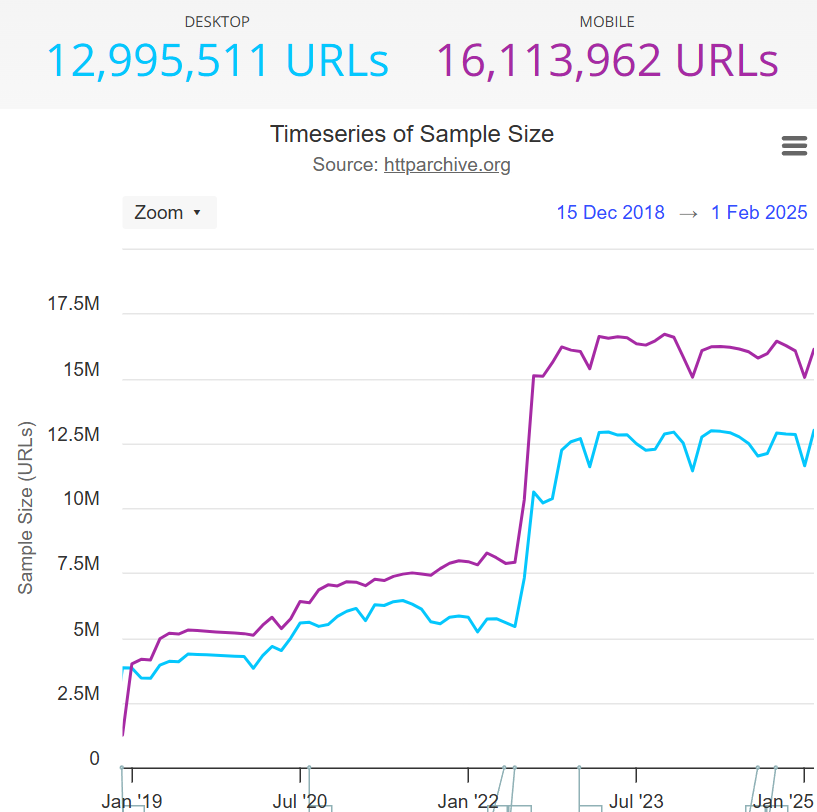
\includegraphics[width=0.4\linewidth]{Gambar/Contoh Sample Size.png}
        \caption{Ukuran sample \web yang digunkan untuk analisis}
        \label{fig:samplesize}
    \end{figure}

        
    \item \textit{Total Kilobytes} yang berisi jumlah dari ukuran perpindahan \textit{kilobytes} dari semua sumber daya yang di \textit{request} oleh halaman \web. Contoh visualisasi data dari laporan ini dapat dilihat pada Gambar~\ref{fig:totalkilo}. Terlihat dari data yang diambil dari 15 Desember 2018 hingga 1 Februari 2025 pada perangkat \desktop dan \mobile bahwa jumlah \textit{kilobyte} yang di\textit{request} tidak mengalami banyak perubahan atau stabil.
    \begin{figure}[H]
        \centering
        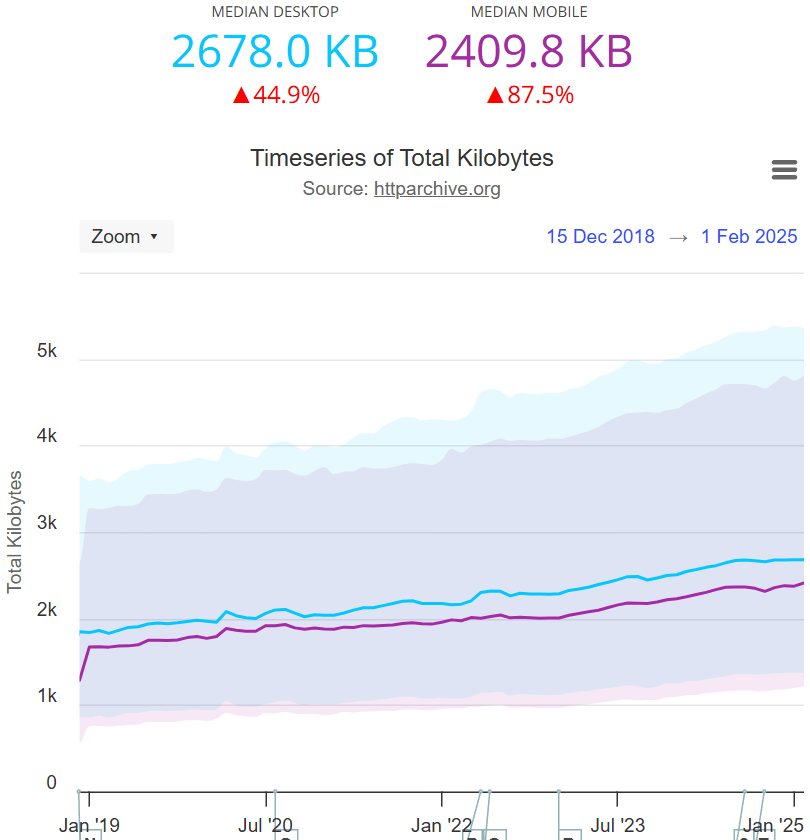
\includegraphics[width=0.4\linewidth]{Gambar/Contoh Total Kilo.png}
        \caption{Total \textit{kilobyte} yang di\textit{request} oleh halaman \web}
        \label{fig:totalkilo}
    \end{figure}

        
    \item \textit{Total Request} yang berisi jumlah\textit{rescource} yang di \textit{request} oleh halaman \web. Contoh hasil visualisasi data dari laporan ini dapat dilihat pada Gambar~\ref{fig:totalrequest}. Terlihat dari data yang diambil dari 15 Desember 2018 hingga 1 Februari 2025 pada perangkat \desktop dan \mobile bahwa pada perangkat \desktop mengalami penurunan yang signifikan pada tanggal 1 april 2019 dengan hanya memiliki satu \textit{request}.
    \begin{figure}[H]
        \centering
        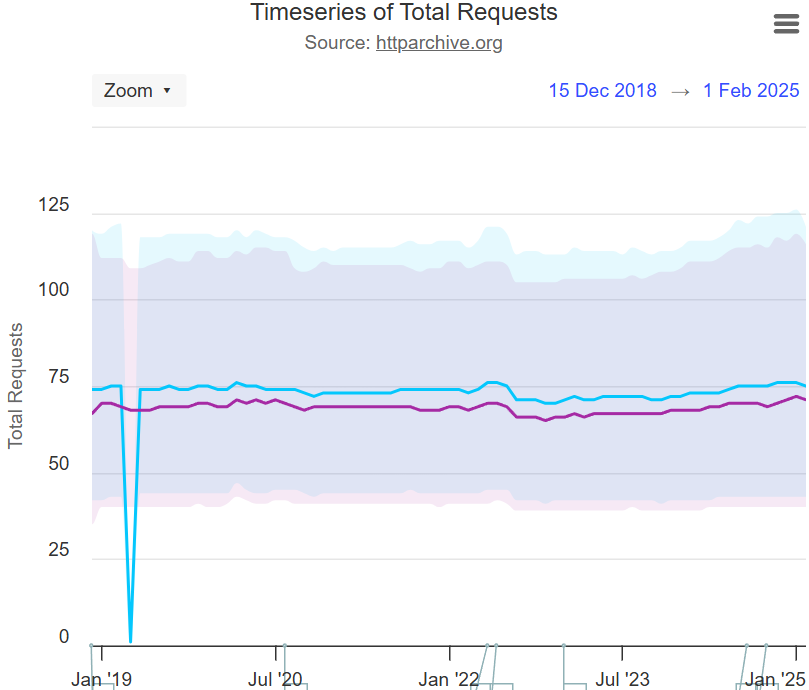
\includegraphics[width=0.4\linewidth]{Gambar/Contoh Total Request.png}
        \caption{Total \textit{Request} yang dilakukan oleh halaman \web}
        \label{fig:totalrequest}
    \end{figure}

    \item \textit{Font Display} yang berisi persentase dari halaman yang menghindari munculnya teks tidak terlihat dengan sekejap sewaktu \web memuat font dengan menggunakan properti CSS \verb|font-display|. Matriks ini diukur dengan menggunakan \light. Contoh visualisasi untuk data ini dapat dilihat pada Gambar~\ref{fig:fontdisp}. Terlihat dari data yang diambil dari 15 Desember 2018 hingga 1 Februari 2025 pada perangkat \desktop dan \mobile bahwa dara untuk perangkat \desktop baru tersedia mulai pada tanggal 1 mei 2022 karena \light baru melakukan migrasi ke perangkat \desktop. Kemudian persentase \web yang menggunakan propreti \verb|font-display| pada perangkat \mobile mengalami penurunan yang signifikan mulai dari tanggal 15 Desember 2018 sampai 1 April 2019 kemudian mengalami kenaikan kembali pada 1 Februari 2021.
    \begin{figure}[H]
        \centering
        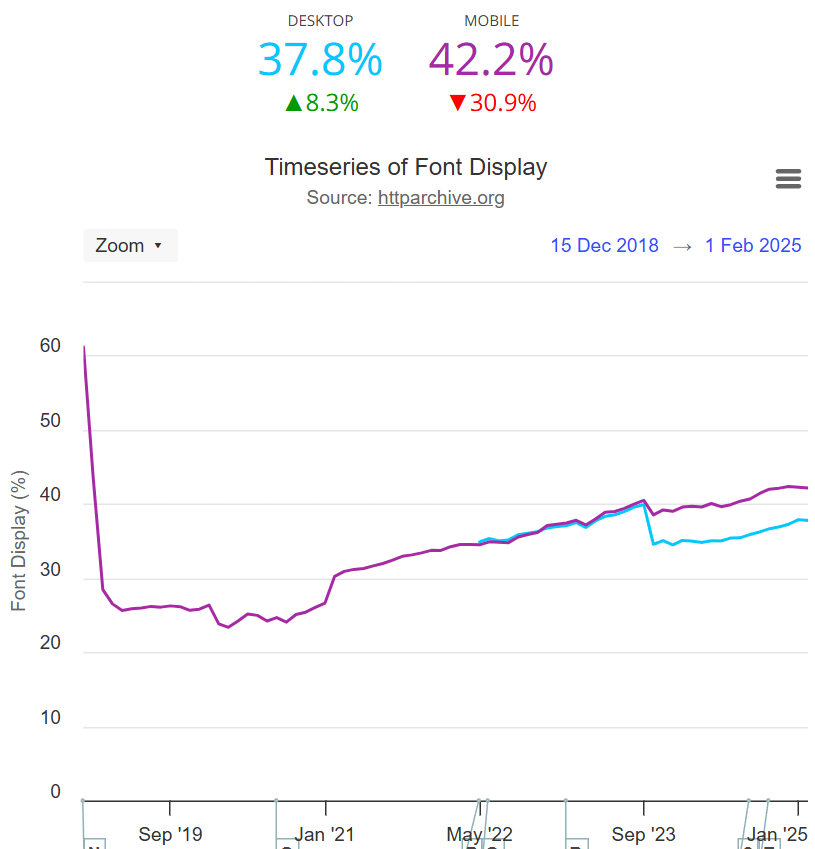
\includegraphics[width=0.4\linewidth]{Contoh Font Display.png}
        \caption{Persentase web yang memiliki properti \texttt{font-display}}
        \label{fig:fontdisp}
    \end{figure}
    
\end{itemize}

\subsubsection{\textit{State of JavaScript}}
\label{subsub:stateofjs}

\textit{JavaScript} membuat halaman \web dapat memiliki aplikasi yang kaya dan lebih interaktif. Laporan dalam kategori ini bertujuan untuk melihat penggunaan \textit{JavaScript} dalam \web dan adopsi serta trennya untuk perangkat \mobile. Report ini akan menganalisis skrip eksternal. Skrip eksternal ini dimaksudkan untuk \textit{resource file} yang menggunakan ekstensi \verb|js| atau \verb|json| atau sebuah tipe MIME((\textit{Multipurpose Internet Mail Extensions}) yang mengandung \verb|script| atau \verb|json|. Beberapa hal yang dianalisis adalah sebagai berikut:
\begin{itemize}
    \item \textit{JavaScript Bytes} yang berisi jumlah ukuran perpindahan \textit{kilobytes} dari skrip eksternal yang di \textit{request}. Contoh visualisasi untuk data ini dapat dilihat pada Gambar~\ref{fig:jsbytes}. Terlihat dari data yang diambil dari 15 Desember 2018 hingga 1 Februari 2025 pada perangkat \desktop dan \mobile bahwa adanya peningkatan \textit{kilobytes} setiap tahun nya. Hal ini menandakan bahwa semakin banyak \textit{resource} yang berbentuk JavaScript yang digunakan oleh halaman \web.
    \begin{figure}[H]
        \centering
        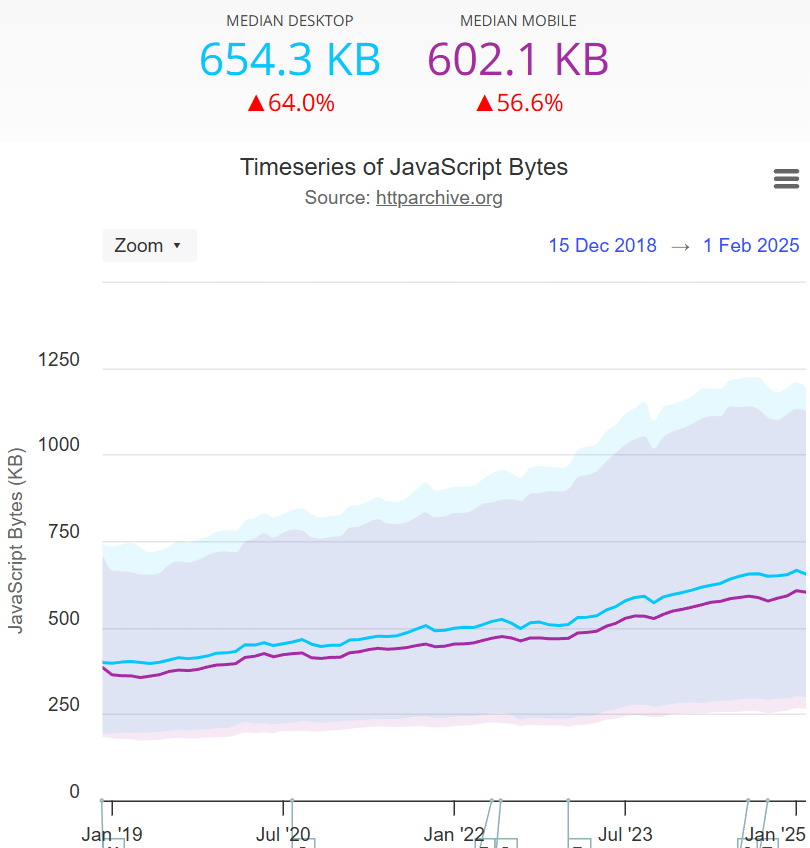
\includegraphics[width=0.4\linewidth]{Gambar/Contoh JavaScript Bytes.png}
        \caption{Jumlah \textit{kilobytes} dari \textit{resource JavaScript}}
        \label{fig:jsbytes}
    \end{figure}

    \item \textit{JavaScript Requests} yang berisi jumlah skrip eksternal yang di \textit{request} oleh halaman \web. Contoh visualisasi dari data ini dapat dilihat pada Gambar~\ref{fig:jsreq}. Terlihat dari data yang diambil dari 15 Desember 2018 hingga 1 Februari 2025 pada perangkat \desktop dan \mobile bahwa jumlah \textit{request} nya cenderung stabil karena tidak adanya kenaikan maupun penurunan jumlah \textit{request} yang signifikan.
    \begin{figure}[H]
        \centering
        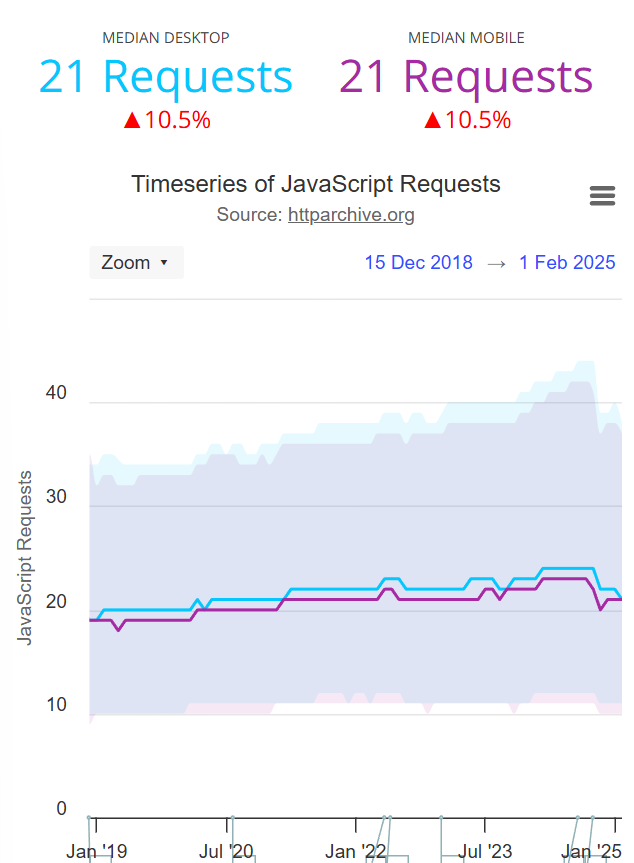
\includegraphics[width=0.4\linewidth]{Gambar/Contoh JavaScript Request}
        \caption{Jumlah Rquest dari \textit{resource} JavaScript}
        \label{fig:jsreq}
    \end{figure}

    
    \item \textit{JavaScript Boot-Up Time} yang berisi jumlah dari waktu CPU yang dibutuhkan oleh setiap \textit{script} di setiap halaman \web. Matriks ini diukur menggunakan \light. Contoh visualisasi dari data ini dapat dilihat pada Gambar~\ref{fig:jsbootup}. Terlihat dari data yang diambil dari 15 Desember 2018 hingga 1 Februari 2025 pada perangkat \desktop dan \mobile bahwa adanya peningkatan jumlah waktu yang dibutuhkan oleh perangkat \mobile. Data untuk perangkat \desktop tidak tercatat secara lengkap karena \light baru melakukan integrasi pada 1 Mei 2022.
    \begin{figure}[H]
        \centering
        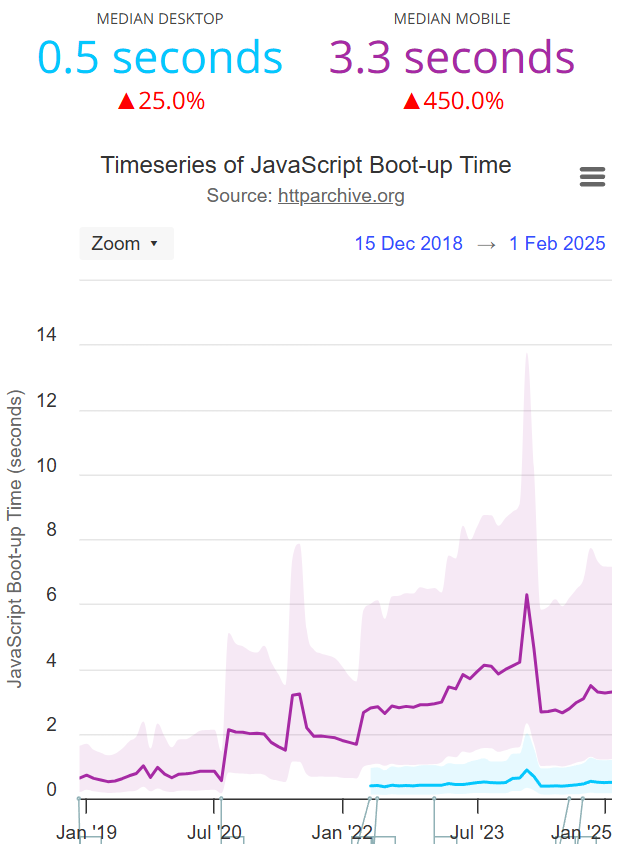
\includegraphics[width=0.4\linewidth]{Gambar/Contoh JavaScript Bootup.png}
        \caption{Perkembangan waktu yang dibutuhkan oleh setiap halaman \web}
        \label{fig:jsbootup}
    \end{figure}
\end{itemize}

\subsubsection{\textit{State of Images}}

\textit{Images} atau gambar merupakan tipe \textit{resource} yang populer digunakan dalam \web. Laporan ini adalah hasil analisa penggunaan gambar eksternal di seluruh \web. Gambar eksternal adalah \textit{resource} yang memiliki ekstensi \verb|png, gif, jpg, jpeg, webp, ico,| atau \verb|svg| atau sebuah tipe MIME((\textit{Multipurpose Internet Mail Extensions}) yang mengandung \verb|image|. Laporan yang masuk kategori ini adalah:
\begin{itemize}
    \item \textit{Image Bytes} yang berisi jumlah ukuran perpindahan \textit{kilobytes} dari gambar eksternal yang di \textit{request} oleh halaman \web. Contoh visualisasi untuk data ini dapat dilihat pada Gambar~\ref{fig:imagesbyte}.Terlihat dari data yang diambil dari 15 Desember 2018 hingga 1 Februari 2025 pada perangkat \desktop dan \mobile bahwa jumlah \textit{kilobytes} yang diperlukan oleh gambar cenderung stabil karena tidak adanya kenaikan atau penurunan yang signifikan.
    \begin{figure}{H}
        \centering
        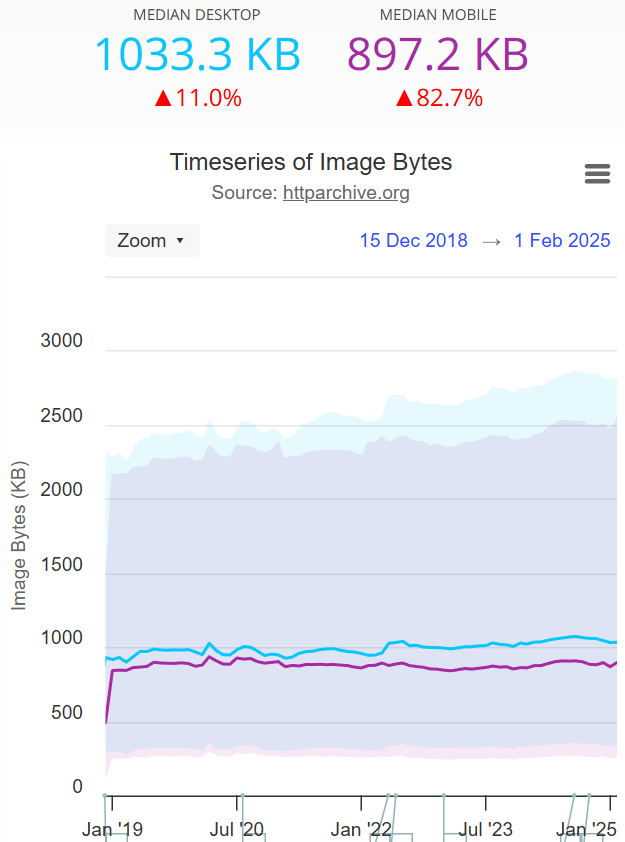
\includegraphics[width=0.4\linewidth]{Gambar/Contoh Image Bytes.png}
        \caption{Perkembangan perpindahan jumlah \textit{kilobytes} yang dibutuhkan oleh gambar}
        \label{fig:imagesbyte}
    \end{figure}

    \item \textit{Image Request} yang berisi jumlah gambar eksternal yang di \textit{request} oleh halaman \web. Hasil visualisasi dari data ini dapat dilihat pada Gambar~\ref{fig:imagerequest}. Terlihat dari data yang diambil dari 15 Desember 2018 hingga 1 Februari 2025 pada perangkat \desktop dan \mobile bahwa jumlah \textit{request} terus mengalami penurunan. Hal ini menandakan bahwa halaman \web mulai mengurangi penggunaan gambar sebagai media untuk menyampaikan informasinya.
    \begin{figure}[H]
        \centering
        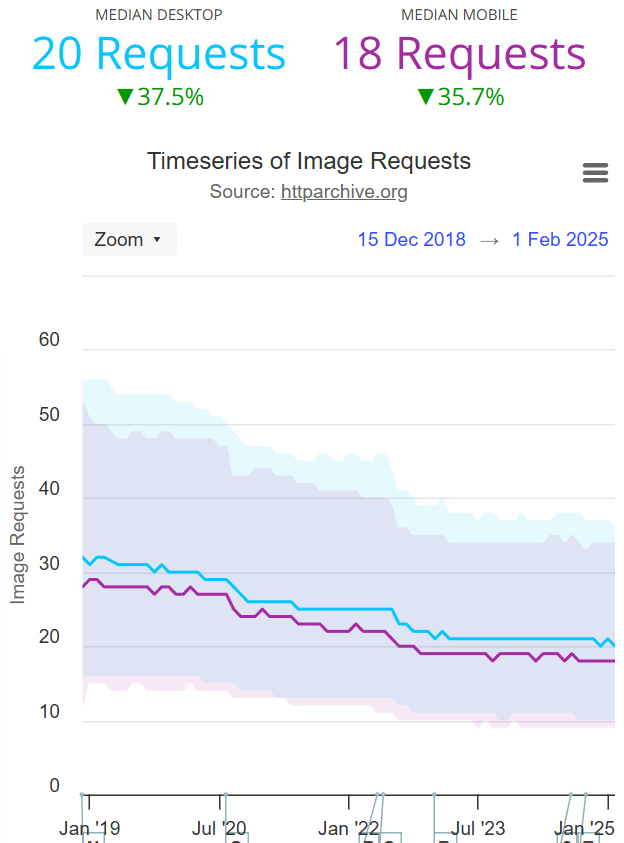
\includegraphics[width=0.4\linewidth]{Gambar/Contoh Image Request.png}
        \caption{Perkembangan jumlah \textit{request} untuk gambar}
        \label{fig:imagerequest}
    \end{figure}

    \item \textit{Offscreen Image Save} yang berisi jumlah \textit{kilobytes} yang dapat dihemat oleh setiap halaman menggunakan \textit{lazy-loading offscreen} dan gambar tersembunyi. Matriks ini berasal dari \light. Hasil visualisasi dari data ini dapat dilihat pada Gambar~\ref{fig:offscreen}. Terlihat dari data yang diambil dari 15 Desember 2018 hingga 1 Februari 2025 pada perangkat \desktop dan \mobile bahwa pada perangkat \mobile jumlah \textit{kilobyte} yang dapat dihemat semakin menurun. Sedangkan pada perangkat \desktop jumlah \textit{kilobyte} yang dapat dihemat cenderung stabil. Data untuk perangkat \desktop dimulai dari 1 Mei 2022 karena \light baru melakukan integrasi dengan perangkat \desktop.
    \begin{figure}[H]
        \centering
        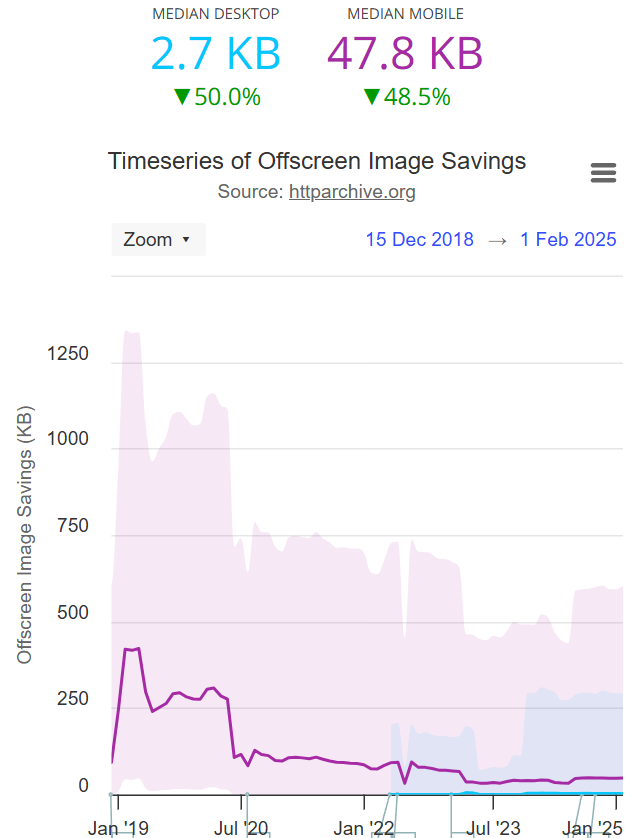
\includegraphics[width=0.4\linewidth]{Gambar/Contoh Hide Image.png}
        \caption{Perkembangan jumlah \textit{kilobyte} yang dapat dihemat dalam penggunaan gambar}
        \label{fig:offscreen}
    \end{figure}
    

    \item \textit{Optimize Image Savings} yang berisi jumlah \textit{kilobytes} yang dapat dihemat oleh setiap halaman dengan mengatur kompresi JPEG ke 85 atau lebih kecil. Contoh visualisasi dari data ini dapar dilihat pada Gambar~\ref{fig:optimizesaving}. Terlihat dari data yang diambil dari 15 Desember 2018 hingga 1 Februari 2025 pada perangkat \desktop dan \mobile bahwa adanya penurunan jumlah \textit{kilobyte}. Pada perangkat \desktop juga mengalami hal yang sama. Hal ini dapat mengindikasikan bahwa pembuat halaman \web tidak memerlukan lagi kompresi pada gambar yang digunankan. Data untuk perangkat \desktop dimulai dari 1 Mei 2022 karena \light baru melakukan integrasi dengan perangkat \desktop.
    \begin{figure}[H]
        \centering
        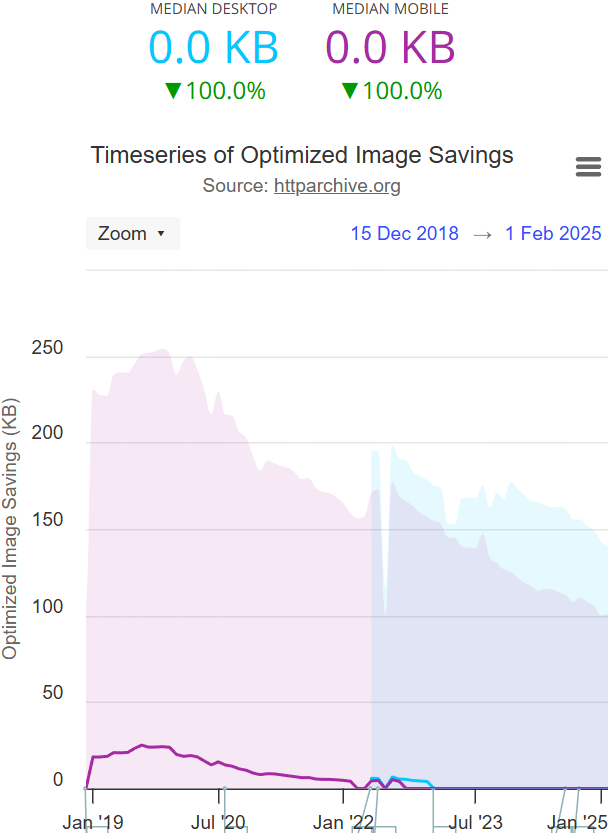
\includegraphics[width=0.4\linewidth]{Gambar/Contoh Optimize Image.png}
        \caption{Perkembangan jumlah \textit{kilobyte yang dapat dihemat dengan melakukan kompresi pada gambar}}
        \label{fig:optimizesaving}
    \end{figure}
\end{itemize}

\subsubsection{\textit{Loading Speed}}
\label{subsub:loading}

Performa \web dapat berpengaruh langsung terhadap bisnis seperti kepuasan pengguna. Laporan ini akan menganalisis berbagai matriks performa dalam siklus pemuatan halaman \web termasuk yang digunakan oleh aplikasi \web modern. Kategori ini memiliki beberapa laporan sebagai berikut:
\begin{itemize}
    \item \textit{First Contentful Paint} yang berisi waktu dalam detik yang dibutuhkan untuk menampilkan konten utama dari sebuah \web ke layar sejak navigasi dimulai. Contoh visualisasi untuk data ini dapat dilihat pada Gambar~\ref{fig:firstcontent}. Terlihat dari data yang diambil dari 15 Desember 2018 hingga 1 Februari 2025 pada perangkat \desktop dan \mobile bahwa adanya penurunan waktu pada perangkat \mobile, ini menjukan bahwa waktu yang dibutuhkan untuk menampilkan kontet utama semakin cepat. Untuk perangkat \desktop waktu yang dibutuhkannya cenderung stabil namun dari visualisasi yang ditunjukan terlihat bahwa perangkat \desktop lebih cepat dalam menampilkan konten utama dibandingkan dengan perangkat \mobile.   
    \begin{figure}[H]
        \centering
        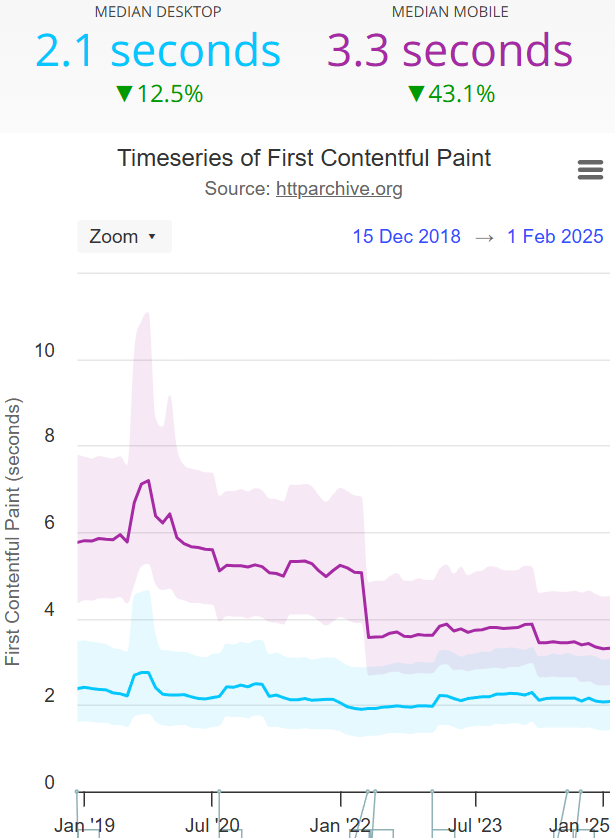
\includegraphics[width=0.4\linewidth]{Gambar/Contoh First Content.png}
        \caption{Perkembangan waktu yang dibutuhkan untuk menampilkan konten utama}
        \label{fig:firstcontent}
    \end{figure}

    \item \textit{Time to interacive} yang berisi waktu yang dibutuhkan agar CPU stabil kembali setidaknya lima detik. Matriks ini diambil dari \light. Contoh visualisasi untuk data ini dapat dilihat pada Gambar~\ref{fig:timeinteractive}. Terlihat dari data yang diambil dari 15 Desember 2018 hingga 1 Februari 2025 pada perangkat \desktop dan \mobile bahwa adanya peningkatan waktu pada perangkat \mobile. Sedangkan untuk perangkat \desktop terlihat penurunan yang signifikan. Data untuk perangkat \desktop dimulai dari 1 Mei 2022 karena \light baru melakukan integrasi dengan perangkat \desktop.
    \begin{figure}[H]
        \centering
        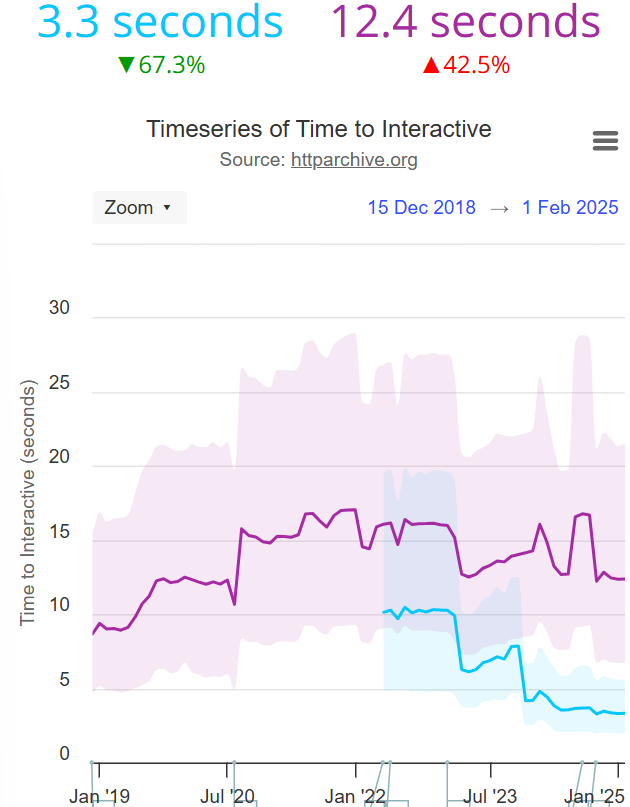
\includegraphics[width=0.4\linewidth]{Gambar/Contoh Time Interactive.png}
        \caption{Perkembangan waktu untuk sebuah \web merespon sebuah navigasi}
        \label{fig:timeinteractive}
    \end{figure}

    \item \textit{JavaScript Boot-up Time} yang berisi jumlah waktu CPU yang dibutuhkan setiap skrip dari setiap halaman. Matriks penilaian ini berasal dari \light. Contoh visualisasi dari data ini dapat dilihat pada Gambar~\ref{fig:jsbootup}. Terlihat dari data yang diambil dari 15 Desember 2018 hingga 1 Februari 2025 pada perangkat \desktop dan \mobile bahwa adanya peningkatan jumlah waktu yang dibutuhkan oleh perangkat \mobile. Data untuk perangkat \desktop tidak tercatat secara lengkap karena \light baru melakukan integrasi pada 1 Mei 2022.


    \item \textit{Speed Index} yang berisi seberapa cepat konten sebuah halaman terlihat secara jelas.  Contoh visualisasi untuk data ini dapat dilihat pada Gambar~\ref{fig:speedindex}. Terlihat dari data yang diambil dari 15 Desember 2018 hingga 1 Februari 2025 pada perangkat \desktop dan \mobile bahwa adanya penurunan waktu yang dibutuhkan oleh perangkat \mobile. Hal ini menunjukan adanya peningkatan kecepatan untuk konten dapat terlihat jelas Sedangkan untuk perangkat \desktop waktu yang dibutuhkan cenderung stabil.
    \begin{figure}[H]
        \centering
        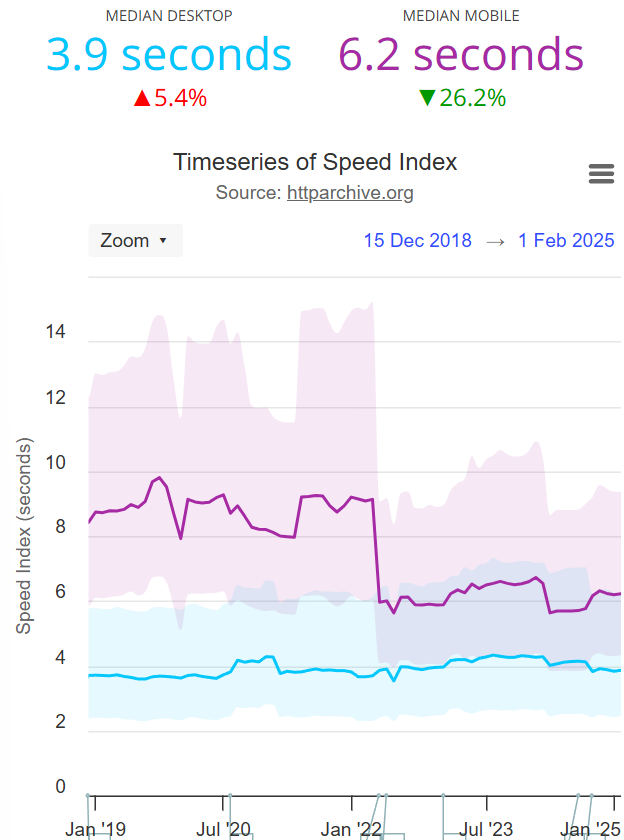
\includegraphics[width=0.4\linewidth]{Gambar/Contoh Speed Index.png}
        \caption{Perkembangan waktu yang dibutuhkan untuk konten dapat terlihat secara jelas}
        \label{fig:speedindex}
    \end{figure}
    
\end{itemize}

\subsubsection{\textit{Progressive Web App}}
\label{subsub:pwa}

Laporan ini akan mengkaji status dari \textit{Progresive Web App}. \textit{Progressive Web App} adalah kelas baru dari aplikasi \web yang disediakan oleh \textit{Service Workers APIs}. \textit{Service Workers} memungkinkan aplikasi untuk mendukung proses muat jaringan secara independen, menerima \textit{push notifications} untuk menyinkronkan data di \textit{background}. Kategori ini mencakup beberapa laporan seperti:
\begin{itemize}
    \item \textit{PWA Scores} yang berisi median dari skor PWA yang terdapat pada \light. Lighthouse adalah alat otomatis yang dapat digunakan untuk meningkatkan performa \web. Contoh visualisasi untuk data ini dapat dilihat pada Gambar~\ref{fig:pwascore}. Terlihat dari data yang diambil dari 15 Desember 2018 hingga 1 Februari 2025 pada perangkat \desktop dan \mobile bahwa skor PWA pada perangkat \mobile mengalami peningkatan. Sedangkan pada perangkat \desktop mengalami penurunan. Data untuk perangkat \desktop tidak tercatat secara lengkap karena \light baru melakukan integrasi pada 1 Mei 2022.
    \begin{figure}[H]
        \centering
        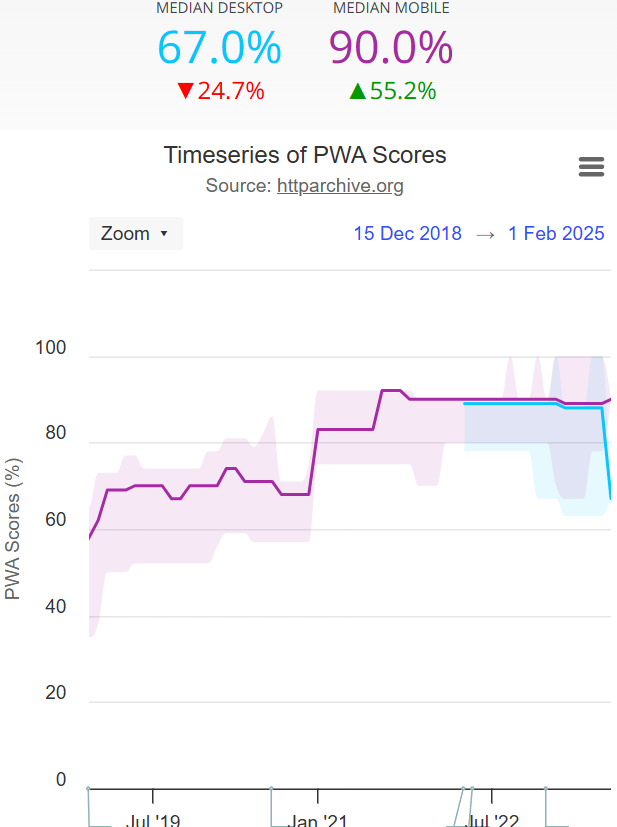
\includegraphics[width=0.4\linewidth]{Gambar/Contoh PWA Score.png}
        \caption{Perkembangan skor PWA}
        \label{fig:pwascore}
    \end{figure}

    \item \textit{Service Worker Controlled Pages} yang berisi persentase dari jumlah halaman yang telah memicu \verb|ServiceWorkerControlledPage| \textit{use counter} yang aktif ketika sebuah halaman \web dikendalikan oleh \textit{service worker}. Contoh visualisasi untuk data ini dapat dilihat pada Gambar~\ref{fig:serverworker}. Terlihat dari data yang diambil dari 15 Desember 2018 hingga 1 Februari 2025 pada perangkat \desktop dan \mobile bahwa adanya peningkatan yang sangat signifikan pada 1 Oktober 2024. Pada titik ini halaman \web yang didukung IPv6 baru ditambahkan. 
    \begin{figure}[H]
        \centering
        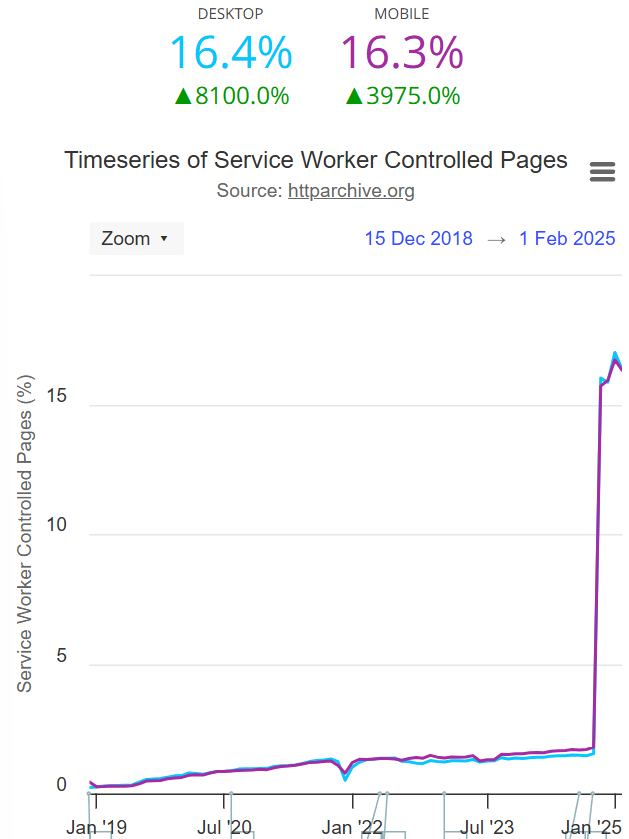
\includegraphics[width=0.4\linewidth]{Gambar/Contoh Service Worker.png}
        \caption{Perkembangan persentase halaman yang membuat \textit{service worker} bekerja}
        \label{fig:serverworker}
    \end{figure}
\end{itemize}


\subsubsection{\textit{Accessibility}}
\label{subsub:access}

Laporan ini menjelaskan tingkat aksesibilitas dari sebuah halaman \web. Penilaian ini dilakukan oleh \light. Kategori ini berisi beberapa laporan seperti:
\begin{itemize}
    \item \textit{Accessibility Score} yang berisi sebaran nilai kategori aksesibilitas dalam \light. Contoh visualisasi untuk data ini dapat dilihat pada Gambar~\ref{fig:accessscore}. Terlihat dari data yang diambil dari 15 Desember 2018 hingga 1 Februari 2025 pada perangkat \desktop dan \mobile bahwa adanya peningkatan pada perangkat \mobile dan \desktop. Hal ini menandakan bahwa halaman \web yang dibuat memiliki tingkat aksesibilitas yang semakin baik. Data untuk perangkat \desktop tidak tercatat secara lengkap karena \light baru melakukan integrasi pada 1 Mei 2022.
    \begin{figure}[H]
        \centering
        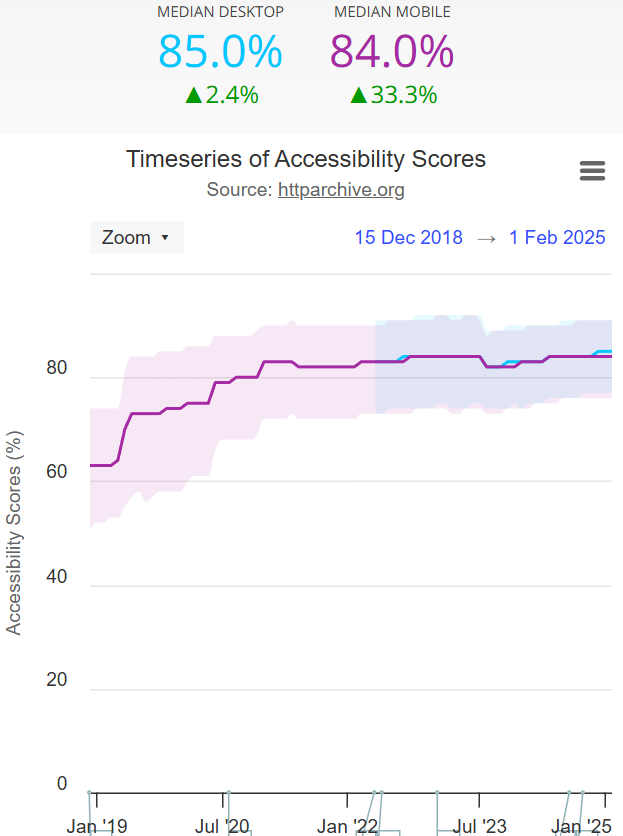
\includegraphics[width=0.4\linewidth]{Gambar/Contoh Accessibility Score.png}
        \caption{Perkembangan persentase skor aksesibilitas}
        \label{fig:accessscore}
    \end{figure}

    \item \textit{Button Name} yang berisi persentase halaman yang berhasil melalui audit \light yang memeriksa apakah \textit{buttons} atau tombol memiliki nama yang aksesibel. Contoh visualisasi untuk data ini dapat dilihat pada Gambar~\ref{fig:buttonname}. Terlihat dari data yang diambil dari 15 Desember 2018 hingga 1 Februari 2025 pada perangkat \desktop dan \mobile bahwa adannya penurunan yang signifikan 1 Agustus 2019 namun kemudian mengalami peningkata di bulan-bulan selanjutnya. Pada perangkat \desktop persentasenya terus meningkat. Hal ini menandakan bahwa nama yang digunakan untuk tombol memiliki tingkat aksesibel yang semakin tinggi. Data untuk perangkat \desktop tidak tercatat secara lengkap karena \light baru melakukan integrasi pada 1 Mei 2022.
    \begin{figure}[H]
        \centering
        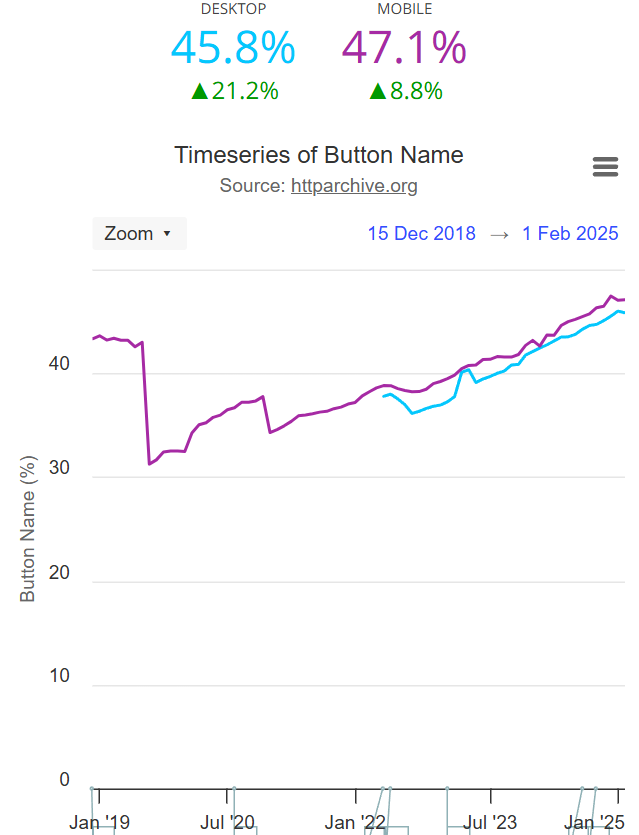
\includegraphics[width=0.4\linewidth]{Gambar/Contoh Button Name.png}
        \caption{Perkembangan persentase \web yang memiliki nama tombol yang aksesibel}
        \label{fig:buttonname}
    \end{figure}

    
    \item \textit{Label} yang berisi persentase halaman yang berhasil melalui audit dari \light yang memeriksa apakah semua elemen memiliki label yang terkait. Contoh visualisasi untuk data ini dapat dilihat pada Gambar~\ref{fig:label}. Terlihat dari data yang diambil dari 15 Desember 2018 hingga 1 Februari 2025 pada perangkat \desktop dan \mobile bahwa adanya peningkatan yang signifikan pada 1 Januari 2021 pada perangkat \mobile. Pada perangkat \desktop persentasenya cenderung stabil. Data untuk perangkat \desktop tidak tercatat secara lengkap karena \light baru melakukan integrasi pada 1 Mei 2022.
    \begin{figure}[H]
        \centering
        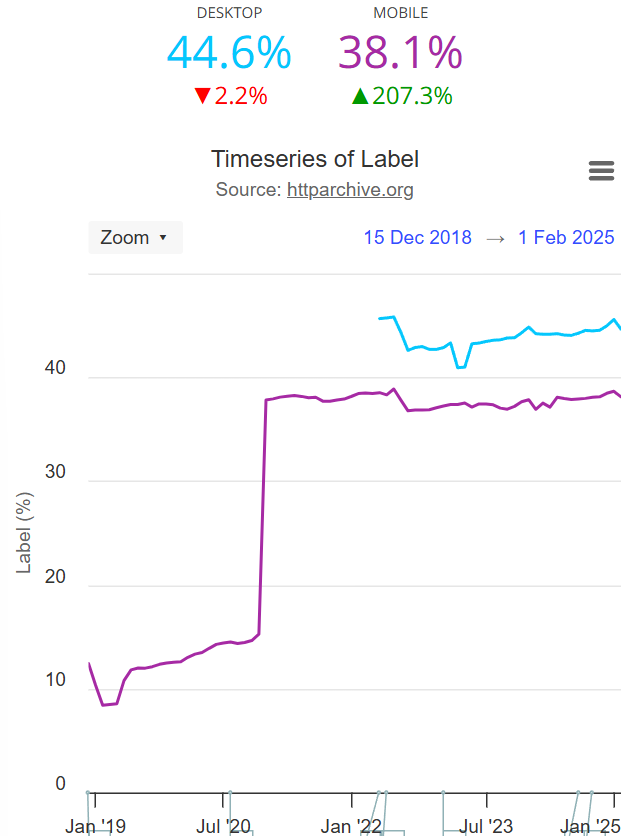
\includegraphics[width=0.4\linewidth]{Gambar/Contoh Label.png}
        \caption{Perkembangan persentase halaman yang menggunakan label yang aksesible}
        \label{fig:label}
    \end{figure}

\end{itemize}


\subsubsection{\textit{SEO}}
\label{subsub:seo}

Laporan yang akan menelusuri penggunaan beberapa teknik agar halaman \web dapat dikenali oleh mesin pencarian secara lebih baik. Kategori ini memiliki beberapa laporan seperti:
\begin{itemize}
    \item rel=canonical yang berisi persentase halaman yang memiliki \textit{link} kanonikal yang valid. Halaman yang kanonikal dideteksi oleh \light. Contoh visualisasi untuk data ini dapat dilihat pada Gambar~\ref{fig:canonical}. Terlihat dari data yang diambil dari 15 Desember 2018 hingga 1 Februari 2025 pada perangkat \desktop dan \mobile bahwa perkembangan halaman yang memiliki \textit{link} yang \textit{canonical} untuk perangkat \desktop dan \mobile cenderung stabil. Data untuk perangkat \desktop tidak tercatat secara lengkap karena \light baru melakukan integrasi pada 1 Mei 2022.
    \begin{figure}[H]
        \centering
        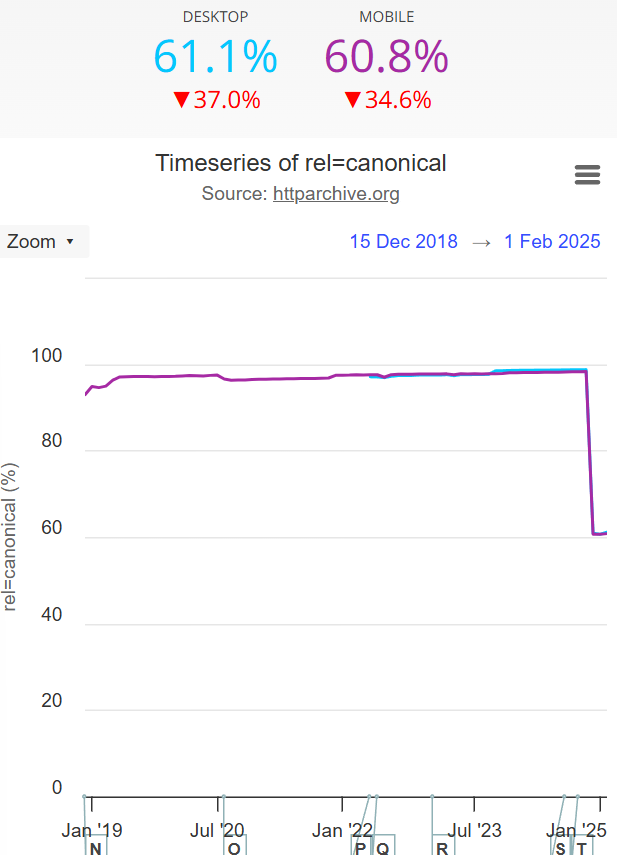
\includegraphics[width=0.4\linewidth]{Gambar/Contoh Canonical.png}
        \caption{Perkembangan persentase halaman yang memiliki \textit{link} \textit{canonical} yang valid}
        \label{fig:canonical}
    \end{figure}

    \item \textit{Descriptive Link Text} yang berisi persentase halaman yang memiliki \textit{link} yang deskriptif. Tingkat \textit{deskriptif} sebuah link diukur oleh \light. Contoh visualisasi untuk data ini dapat dilihat pada Gambar~\ref{fig:disclink}. Terlihat dari data yang diambil dari 15 Desember 2018 hingga 1 Februari 2025 pada perangkat \desktop dan \mobile bahwa persentase halaman yang memiliki link deskriptif cenderung stabil. 
    \begin{figure}[H]
        \centering
        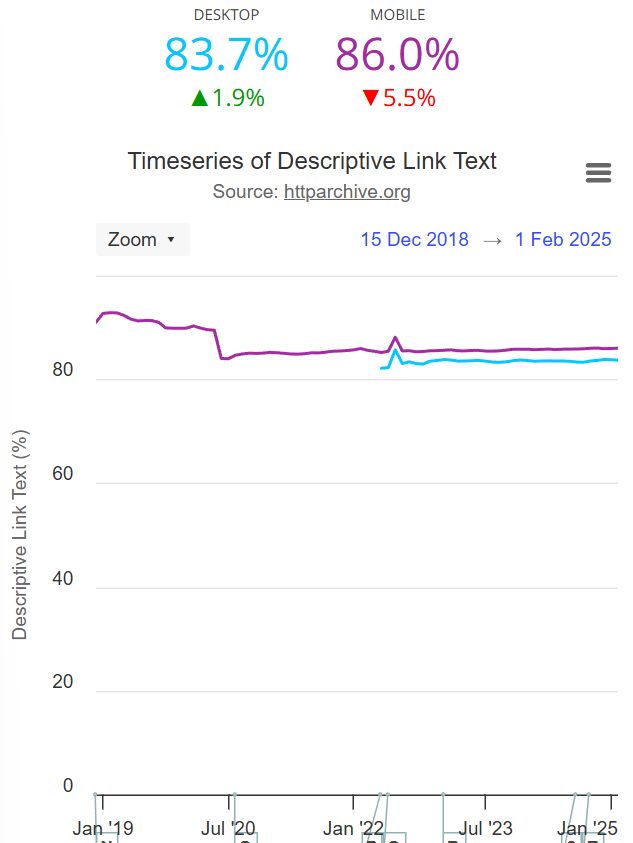
\includegraphics[width=0.4\linewidth]{Gambar/Contoh Descriptive Link.png}
        \caption{Perkembangan persentase halaman yang memiliki \textit{link} yang deskriptif}
        \label{fig:disclink}
    \end{figure}
\end{itemize}

\subsubsection{\textit{Page Weight}}
\label{subsub:pageweight}

Laporan ini menelusuri ukuran dan banyaknya \textit{resource} dari banyak halaman \web populer. Ukuran dalam hal ini merepresentasikan jumlah \textit{byte} yang dikirimkan melalui jaringan. Kategori ini memiliki beberapa laporan seperti:
\begin{itemize}
    \item \textit{Total Kilobytes} yang berisi jumlah kilobyte dari semua resource yang diminta oleh halaman \web. Contoh visualisasi untuk data ini dapat dilihat pada Gambar~\ref{fig:totalkilo}. Terlihat dari data yang diambil dari 15 Desember 2018 hingga 1 Februari 2025 pada perangkat \desktop dan \mobile bahwa jumlah \textit{kilobyte} yang di\textit{request} tidak mengalami banyak perubahan atau stabil.

    \item \textit{JavaScript Bytes} yang berisi jumlah kilobyte yang diminta oleh skrip eksternal dari sebuah halaman \web. Contoh visualisasi untuk data ini dapat dilihat pada Gambar~\ref{fig:jsbytes}. Terlihat dari data yang diambil dari 15 Desember 2018 hingga 1 Februari 2025 pada perangkat \desktop dan \mobile bahwa adanya peningkatan \textit{kilobytes} setiap tahun nya. Hal ini menandakan bahwa semakin banyak \textit{resource} yang berbentuk JavaScript yang digunakan oleh halaman \web.

    \item \textit{HTML Bytes} yang berisi jumlah kilobyte yang diminta oleh dokumen HTML dari sebuah halaman \web.  Contoh visualisasi untuk data ini dapat dilihat pada Gambar~\ref{fig:htmlreq}. Terlihat dari data yang diambil dari 15 Desember 2018 hingga 1 Februari 2025 pada perangkat \desktop dan \mobile bahwa jumlah \textit{kilobytes} pada perangkat \mobile dan \desktop mengalami peningkatan namun meningkat secara perlahan.
    \begin{figure}[H]
        \centering
        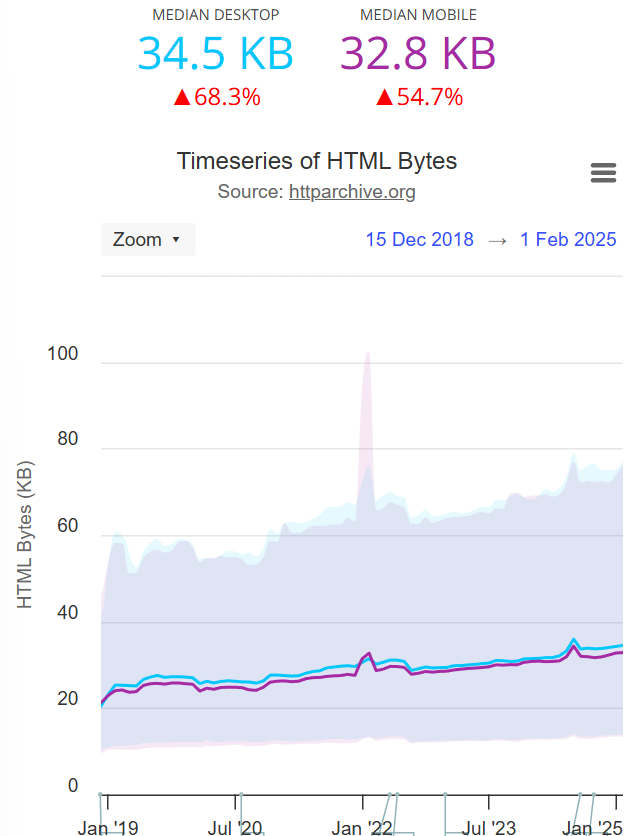
\includegraphics[width=0.4\linewidth]{Gambar/Contoh HTML Bytes.png}
        \caption{PErkembangan jumlah \textit{kilobytes} oleh dokumen HTML}
        \label{fig:htmlreq}
    \end{figure}

\end{itemize}

\subsubsection{\textit{CrUx}}
\label{subsub:crux}

Laporan ini akan menelusuri tingkat interaktivitas dan proses muat dari pengguna \textit{Chrome} di dunia nyata melalui berbagai kondisi perangkat keras dan jaringan. Kategori ini memiliki beberapa laporan seperti:
\begin{itemize}
    \item \textit{Passes Core Web Vitals} yang bersisi persentase halaman \web yang berhasil lolos degan penilaian baik dari tiga matriks penilaian \textit{Core Web Vitals}. Contoh visualisasi untuk data ini dapat dilihat pada Gambar~\ref{fig:cwvpass}. Terlihat dari data yang diambil dari 1 Desember 2018 hingga 1 Februari 2025 pada perangkat \desktop dan \mobile bahwa pada perangkat \desktop dan \mobile mengalami peningkatan. Ini menunjukan bawha kualitas halaman \web semakin baik.
    \begin{figure}[H]
        \centering
        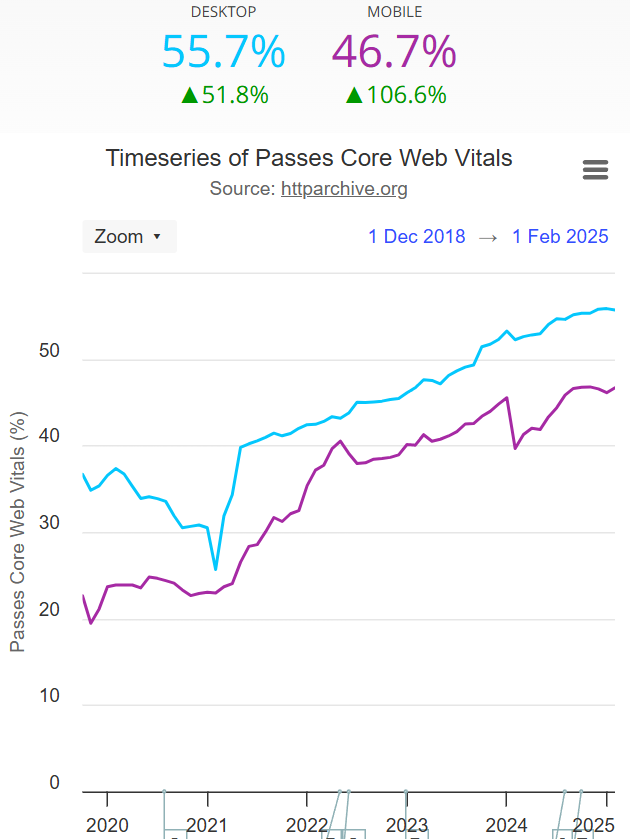
\includegraphics[width=0.4\linewidth]{Gambar/Contoh Core Web Pass.png}
        \caption{Perkembangan oersentase halaman \web yang memiliki penilaian \textit{core web vitalis} yang bagus}
        \label{fig:cwvpass}
    \end{figure}

    \item \textit{Good First Paint} yang berisi persentase halaman \web yang memiliki pengalaman \textit{First Paint} yang ``baik''. Waktu yang dikatakan baik adalah saat halaman \web mendapat skor FP kurang dari sama dengan satu detik. Contoh visualisasi untuk data ini dapat dilihat pada Gambar~\ref{fig:firstpaint}. Terlihat dari data yang diambil dari 1 Desember 2018 hingga 1 Februari 2025 pada perangkat \desktop dan \mobile bahwa persentase halaman yang memiliki penilaian yang baik meningkat. Hal ini menunjukan bahwa semakin banyak halaman \web memiliki pengalaman \textit{First Paint} yang baik. 
    \begin{figure}[H]
        \centering
        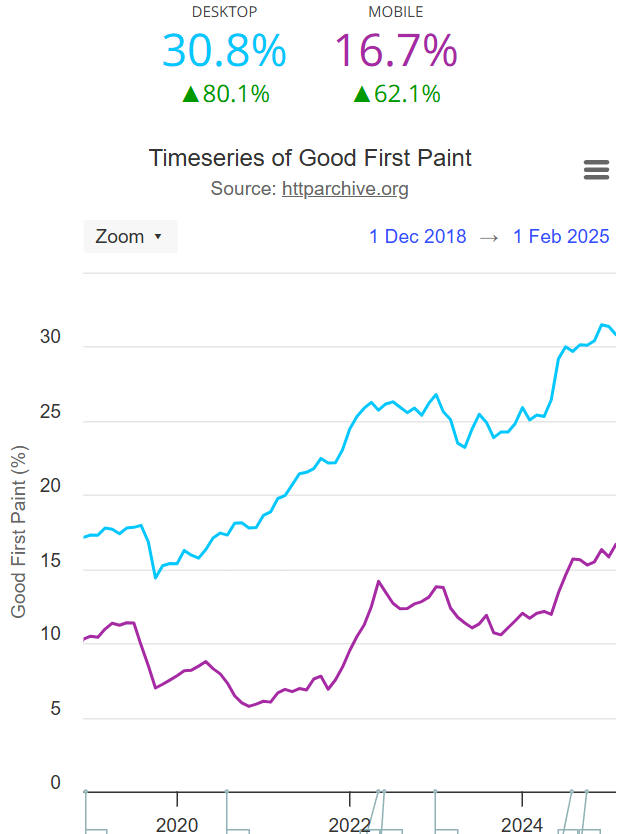
\includegraphics[width=0.4\linewidth]{Gambar/Contoh Good Paint.png}
        \caption{Contoh perkembangan persentase halaman yang memiliki pengalaman \textit{First Paint} yang baik}
        \label{fig:firstpaint}
    \end{figure}

    \item \textit{Good DOM Content Loaded} yang berisi persentase halaman \web yang memiliki pengalaman DCL(\verb|DOMContentLoaded|) yang ``baik''. NIlai yang dikatakan baik adalah halamanya yang berhasil dimuat kurang dari sama dengan satu detik. Contoh visualisasi untuk data ini dapat dilihat pada Gambar~\ref{DCL}. Terlihat dari data yang diambil dari 1 Desember 2018 hingga 1 Februari 2025 pada perangkat \desktop dan \mobile bahwa adanya peningkatan persentase halaman \web yang memiliki pengalaman DCL yang baik pada perangkat \desktop dan \mobile. 
    \begin{figure}[H]
        \centering
        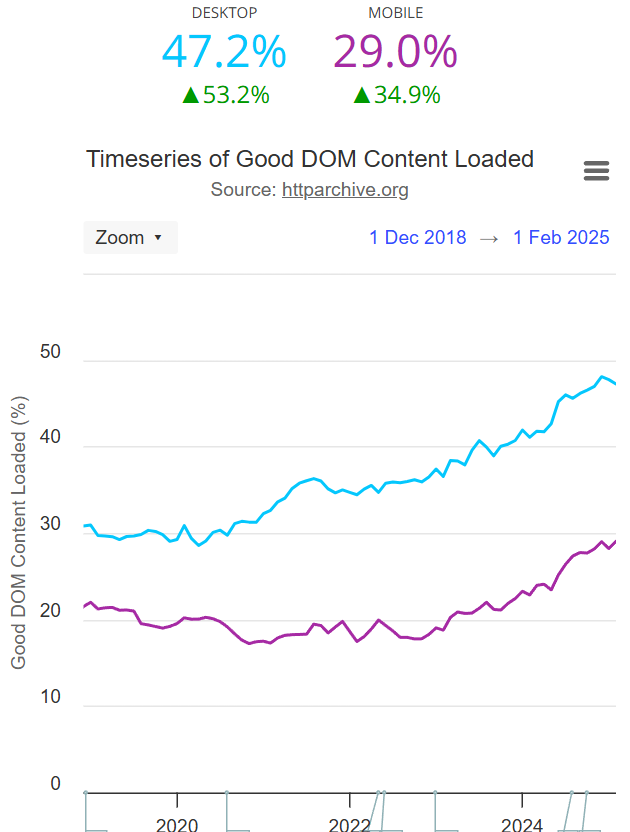
\includegraphics[width=0.4\linewidth]{Gambar/Contoh DOM.png}
        \caption{Contoh perkembangan persentase halaman \web yang memiliki pebgalaman DCL yang baik}
        \label{fig:DCL}
    \end{figure}
\end{itemize}

\subsubsection{\textit{Capabilities}}
\label{subsub:capable}

\textit{Capabilities Project} adalah usaha yang dilakukan oleh \textit{Google} dengan perusahaan lain untuk memungkinkan sebuah aplikasi \web dapat melakukan hal yang dapat dilakukan oleh aplikasi bawaan dari sistem operasi sambil tetap mempertahankan keamanan pengguna, privasi, kepercayaan, dan prinsip dasar lainnya dari \web. Kategori ini memiliki beberapa laporan seperti:
\begin{itemize}
    \item \textit{Async Clipboard Read} yang berisi persantase halaman yang membaca data dari \textit{clipboard} yang dimiliki sistem melalui API \textit{Async Clipboard}. Contoh visualisasi untuk data ini dapat dilihat pada Gambar~\ref{fig:async}. Terlihat dari data yang diambil dari 15 Desember 2018 hingga 1 Februari 2025 pada perangkat \desktop dan \mobile bahwa perkembangannya sangat tidak stabil karena hasil visualisasinya memperlihatkan garus yang naik turun secara ekstrem.
    \begin{figure}[H]
        \centering
        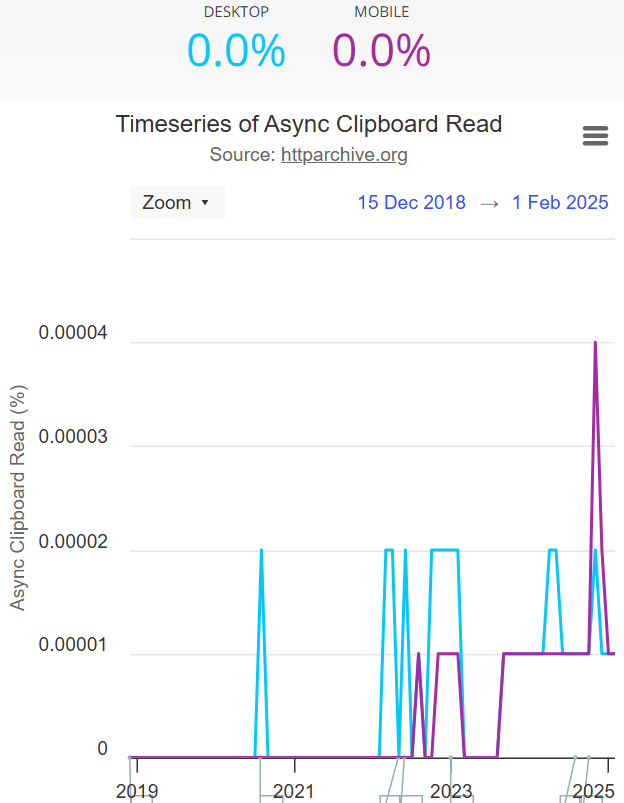
\includegraphics[width=0.4\linewidth]{Gambar/Contoh Async.png}
        \caption{Perkembangan persentase halaman \web yang membaca \textit{clipboard} milik sistem.}
        \label{fig:async}
    \end{figure}
    

    \item \textit{Notification Triggers} yang berisi persentase halaman yang menggunakan pemberitahuan terjadwal dengan menggunakan API \textit{Notification Trigger}. Contoh visualisasi untuk data ini dapat dilihat pada Gambar~\ref{fig:notif}. Terlihat dari data yang diambil dari 15 Desember 2018 hingga 1 Februari 2025 pada perangkat \desktop dan \mobile bahwa tidak ada halaman \web yang menggunakan API \textit{Notification Trigger}.
    \begin{figure}[H]
        \centering
        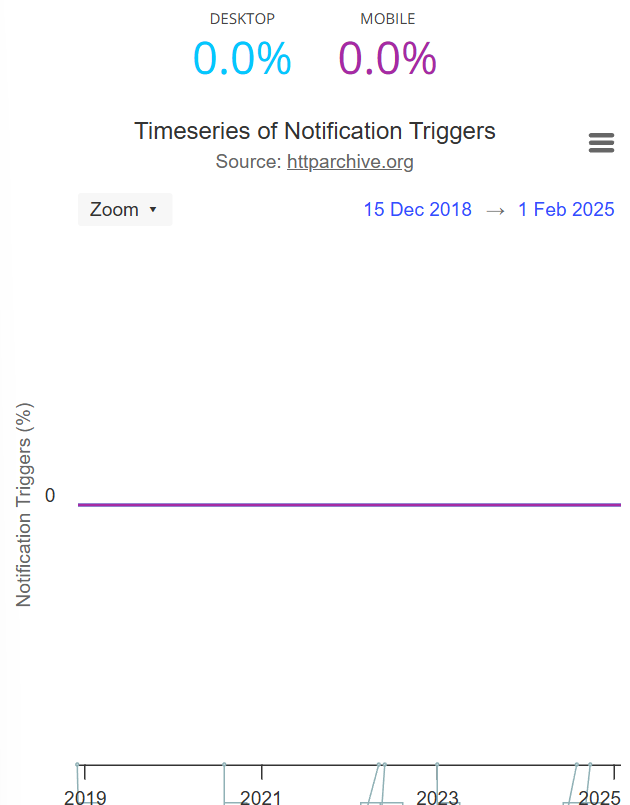
\includegraphics[width=0.4\linewidth]{Gambar/Contoh Notif.png}
        \caption{Perkembangan penggunaan API \textit{Notification Trigger}}
        \label{fig:notif}
    \end{figure}

    \item \textit{Idle Detection} yang berisi persentase halaman yang mendeteksi penggunanya sedang melakukan \textit{idle} melalui API \textit{Idle Detection}. Contoh visualisasi untuk data ini dapat dilihat pada Gambar~\ref{fig:idle}. Terlihat dari data yang diambil dari 15 Desember 2018 hingga 1 Februari 2025 pada perangkat \desktop dan \mobile bahwa persentase halaman yang menggunakan API ini sangat fluktuatif. Hal ini ditunjukan dari bentuk visualisasi yang menunjukan peningkatan dan penurunan dalam waktu yang cepat dan sangat ekstrem.
    \begin{figure}[H]
        \centering
        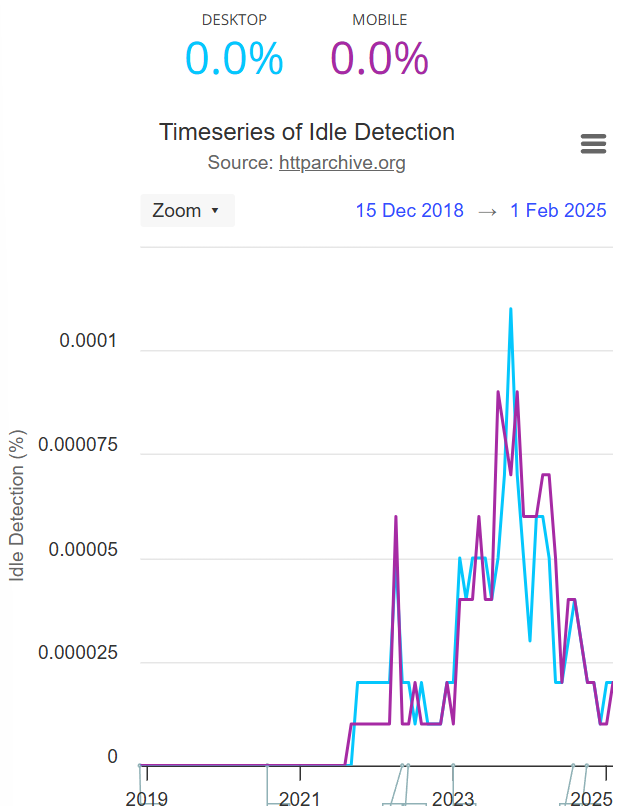
\includegraphics[width=0.4\linewidth]{Gambar/Contoh Idle.png}
        \caption{Perkembangan persentase halaman \web penggunaan API \textit{Idle Detection}}
        \label{fig:idle}
    \end{figure}
\end{itemize}


\subsubsection{\textit{Core Web Vitals Technology Report}}
\label{subsub:cwv}
Laporan \textit{Core Web Vitalis Technology} merupakan dasbor yang berisi gabungan dari pengalaman nyata pengguna \textit{chrome}(CrUX) dengan pendeteksi teknologi \web yang dimiliki \http, yang memungkinkan analisis terhadap cara sebuah \web dibangun dan pengalaman saat \web tersebut digunakan. Kategori ini memiliki beberapa laporan seperti:
\begin{itemize}
    \item \textit{Technology Drilldown} yang berisi informasi yang lebih detail mengenai satu teknologi. Contoh visualisasi untuk data ini dapat dilihat pada Gambar~\ref{fig:techdrill}. Terlihat dari data yang diambil dari 15 Desember 2018 hingga 1 Februari 2025 pada perangkat \desktop dan \mobile bahwa persentase halaman yang memiliki skor CWV yang baik dengan menggunakan teknologi \textit{WordPress} semakin meningkat.
        \begin{figure}[H]
            \centering
            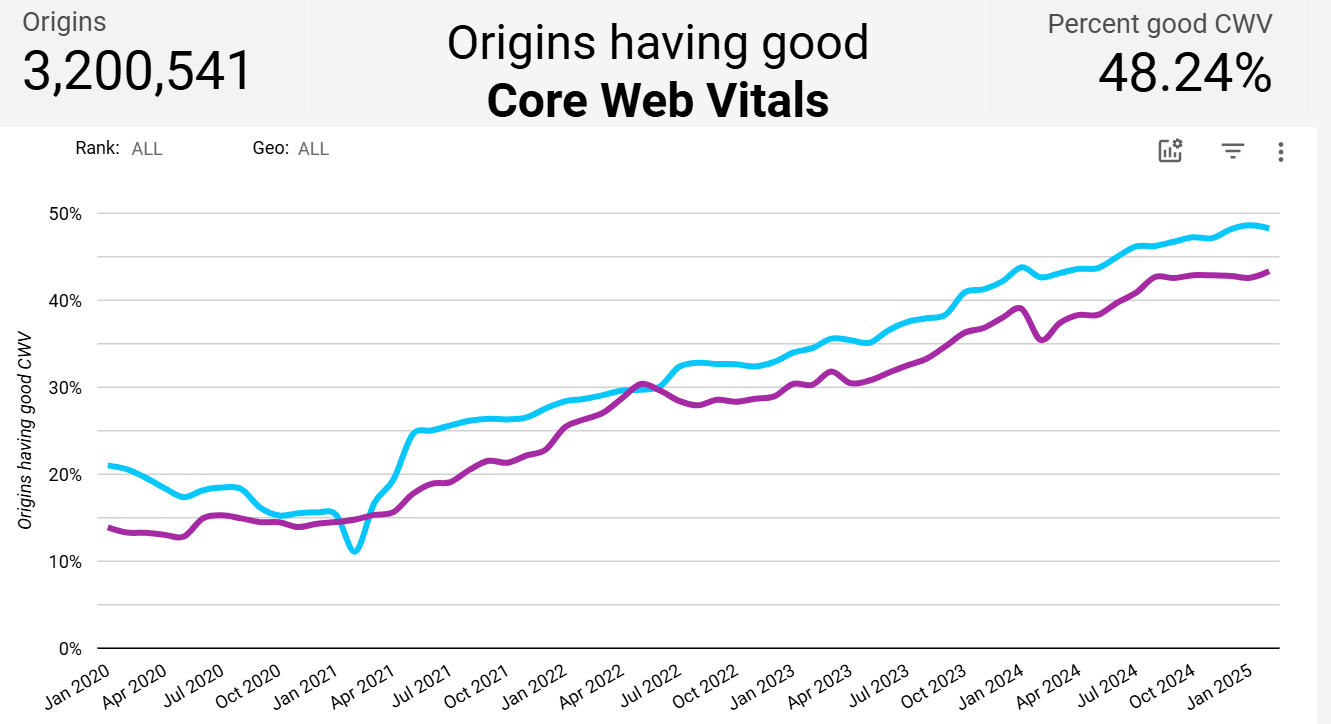
\includegraphics[width=0.4\linewidth]{Gambar/Contoh TechDrill.png}
            \caption{Perkembangan persentase halaman \web yang menggunakan teknologi \textit{WordPress} dengan skor CWV yang baik}
            \label{fig:techdrill}
        \end{figure}

    \item \textit{Technology Comparasion} yang bersi informasi yang lebih detail mengenai dua sampai sepuluh teknologi. Contoh visualisasi untuk data ini dapat dilihat pada Gambar~\ref{fig:techcompar}. Terlihat dari data yang diambil dari 15 Desember 2018 hingga 1 Februari 2025 pada perangkat \mobile bahwa semua teknoligi memiliki peningkatan skor CWV yang baik.
        \begin{figure}[H]
            \centering
            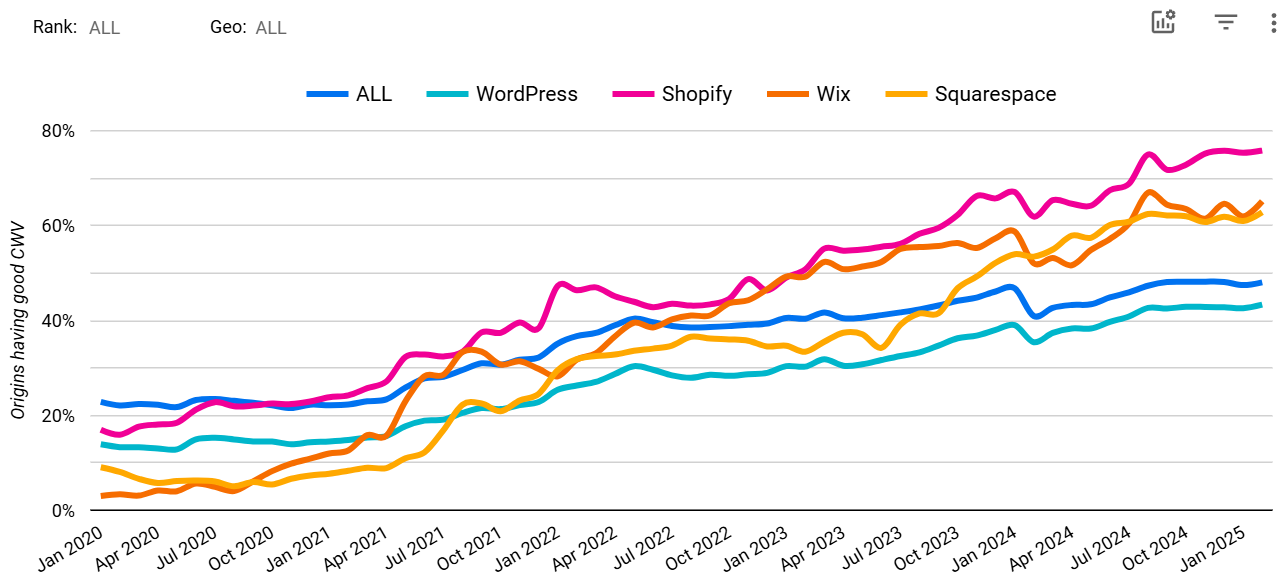
\includegraphics[width=0.4\linewidth]{Gambar/Contoh Tech Compar.png}
            \caption{Perkembangan persentase halaman \web yang memiliki skor CWV yang bagus dengan berbagai teknologi}
            \label{fig:techcompar}
        \end{figure}

    \item \textit{Category} yang berisi informasi yang lebih detail mengenai sebuah kategori dan teknologi yang dimilikinya.
\end{itemize}


\subsection{2024 \textit{Web Almanac}}
\label{subsec:almanac}

\textit{Web Almanac} merupakan kombinasi dari statistik yang masih mentah dan tren yang ada di \http dengan keahlian komunitas \web. \textit{Web Almanac} memiliki 19 bab yang berisi hal berikut ini:
\begin{enumerate}
    \item \textit{JavaScript} Bab yang berisi hasil evaluasi peran \textit{JavaScript} dalam dunia \web. 
    \item \textit{Markup} Bab yang berisi tentang analisis dari halaman HTML yang dimiliki oleh \web yang dievaluasi.
    \item \textit{Structured Data} Bab yang berisi hasil analisis tren di tahun lalu dan memeriksa perkembanan cepat yang terjadi.
    \item \textit{Fonts} Bab yang berisi hasil analisis penggunaan \textit{web font}.
    \item \textit{Media} Bab yang berisi hasil analisis tentan HTTP/1.1, HTTP/2 and HTTP/3 manajemen media seperti video dan gambar.
    \item \textit{Third Parties} Bab yang berisi hasil analisis empiris yang menjelaskan praktik penggunaan pihak ketika ada \web.
    \item \textit{SEO} Bab yang menjelaskan mengenai elemen dan pengaturan yang penting agar \web dapat terlihat pada pencarian.
    \item \textit{Accessibility} Bab yang berisi solusi yang ditawarkan agar memiliki tingkat aksesibilitas yang baik.
    \item \textit{Performance} Bab yang berisi hasil analisis peforma berdasarkan skor \textit{core web vitals}.
    \item \textit{Privacy} Bab yang berisi ringkasan mengenai \textit{online tracking}. 
    \item \textit{Security} Bab yang berisi hasil analisis proteksi dan praktek keamanan yang digunakan oleh halama \web saat ini.
    \item \textit{CMS} Bab yang berisi hasil analisis terhadap varasi darin sistem manajemen konten yang dimiliki berbagai halaman \web.
    \item \textit{Ecommerce} Bab yang berisi ringkasan mengenai ekosistem \textit{e-commerce} dalam \web 
    \item \textit{JamStack} Bab yang berisi analisis mengenai penggunaan tiga arsitektur halamany yang digunakan pada \web.
    \item \textit{Sustainability} Bab yang berisi bagaiman mengurangi dampak dari ekosistem \web terhadap lingkungan.
    \item \textit{Page Weight} Bab yang berisi hasil analisis terhadap bobot halaman yang dapat dibuka oleh semua pengguna dalam berbagai kondisi.
    \item \textit{CDN} Bab yang berisi hasil kajian terhadap \textit{Content Delivery Network} dan peran pentingnya dalam ekosistem digital saat ini.
    \item \textit{HTTP} Bab yang berisi hasil analaisis penggunaan HTTP/1.1, HTTP/2, dan HTTP/3 serta perkembanganya saat ini.
    \item \textit{Cookies} Bab yang berisi hasil analaisis struktur \textit{cookie} dari halaman \web.
\end{enumerate}

Metode yang digunakan oleh \http dalam mengumpulkan data perkembangan pembuatan \web sejak 2010 adalah dengan menggunakan \textit{WebPageTest} dan \light. \light adalah sebuah alat \textit{open-source} yang disediakan oleh \textit{Google} untuk meningkatkan kualitas halaman \web~\cite{lighthouse}. \light dapat melakukan pemeriksaan terhadap performa, aksesibilitas, dan SEO(\textit{Search Engine Optimization}) dari sebuah halaman \web.

\subsection{\textit{Public Dataset}}
\label{subsec:pd}
\http memberikan akses terhadap informasi yang lebih detail mengenai hal-hal yang ada di setiap \textit{website}, seperti \textit{metadata} dari \textit{request} dan \textit{response}, \textit{response bodies}, jejak eksekusi, dan lain-lain. \http memberikan beberapa tabel yang terbagi kedalam beberapa \textit{dataset} seperti \textit{crawl, sample\_data}, dan \textit{wappalyzer}. Dataset sendiri adalah unit logis utama untuk mengelompokan dan mengatur \textit{view, resource}, dan tabel pada \textit{Google BigQUery} dataset-dataset tersebut kemudian memiliki beberapa tabel yang dapat digunakan seperti berikut ini:

\begin{itemize}
    \item \textit{pages} adalah tabel yang terdapat pada dataset \textit{crawl} dan berisi detail mengenai halaman yang dites oleh \http. Data ini memiliki kolom sebagai berikut:
    \begin{itemize}
        \item \textit{date}
        \item \textit{client}
        \item \textit{page}
        \item \textit{is\_root\_page}
        \item \textit{root\_page}
        \item \textit{rank}
        \item \textit{wptid}
        \item \textit{payload}
        \item \textit{summary}
        \item \textit{custom\_metric}
        \item \textit{lighthouse}
        \item \textit{features}
        \item \textit{technologies}
        \item \textit{metadata}
    \end{itemize}
    
    \item \textit{pages\_10k} adalah tabel yang terdapat pada \textit{dataset sample\_data} yang merupakan potongan dari tabel \textit{pages} pada \textit{dataset crawl} yang berisi halaman-halaman yang dites dan memiliki peringkat popularitas diatas 10.000 berdasarkan CrUX. Tabel ini memiliki kolom sebagai berikut:
    \begin{itemize}
        \item \textit{date}
        \item \textit{client}
        \item \textit{page}
        \item \textit{is\_root\_page}
        \item \textit{root\_page}
        \item \textit{rank}
        \item \textit{wptid}
        \item \textit{payload}
        \item \textit{summary}
        \item \textit{custom\_metric}
        \item \textit{lighthouse}
        \item \textit{features}
        \item \textit{technologies}
        \item \textit{metadata}
    \end{itemize}

    \item \textit{requests} adalah tabel yang terdapat pada \textit{dataset crawl} yang berisi detail \textit{request} dari halaman yang diuji oleh \http. TAbel ini memiliki kolom sebagai berikut:
    \begin{itemize}
         \item \textit{date}
        \item \textit{client}
        \item \textit{page}
        \item \textit{is\_root\_page}
        \item \textit{root\_page}
        \item \textit{url}
        \item \textit{is\_main\_document}
        \item \textit{type}
        \item \textit{index}
        \item \textit{payload}
        \item \textit{summary}
        \item \textit{request\_header}
        \item \textit{reponse\_header}
        \item \textit{response\_ body}
    \end{itemize}

    
    \item \textit{technologies}  adalah tabel yang berisi \textit{dataset wappalyzer} yang berisi mengenai detail dari teknologi yang dipakai oleh berbagai \web. Tabel ini memiiliki tabel sebagai berikut:
     \begin{itemize}
        \item \textit{technologies}
        \item \textit{categories}
        \item \textit{info}
    \end{itemize}

\end{itemize}


\section{\textit{Structure Query Language}~\cite{book:SQLBigQuery}}
\label{sec:sql} 
\textit{Structure Query Language} atau yang biasa disebut SQL merupakan bahasa pemrograman yang bertujuan untuk menganalisi dan mengolah basis data relasional. Lakshman dalam bukunya menjelaskan bahwa SQL sangat cocok digunakan dalam lingkungan analitik yang besar seperti dalam lingkungan \textit{Big Query}. Sintaks yang dapat dipakai adalah sebagai berikut:
\begin{itemize}
    \item \verb|SELECT| dan \verb|FROM| merupakan sintaks yang berguna untuk memilih bagian data yang dibutuhkan dari tabel tertentu. Sintaks ini digunakan dengan cara \verb|SELECT nama, kolom FROM nama.tabel|
    \begin{lstlisting}[language=SQL, caption=contoh penggunaan sintaks \lstinline|SELECT|, label=kode:contohselect]
        SELECT
            date, client
        FROM
            `httparchive.crawl.pages`
    \end{lstlisting}
    Kueri pada potongan Kode~\ref{kode:contohselect} akan mengembalikan tabel yang berisi kolom \textit{date} dan \textit{client} dari tabel \textit{httparchive.crawl.pages}.
    
    \item \verb|WHERE| adalah sintaks yang berguna untuk memberikan kondisi tertentu dalam memilih data. Kondisi yang diinginkan bisa lebih dari satu maka dari itu untuk menggabungkan beberapa kondisi dapat digunakan fungsi \verb|AND|, \verb|OR|, atau \verb|BETWEEN|. Sintaks ini digunakan dengan cara \verb|SELECT nama, kolom FROM nama.tabel WHERE kondisi1 AND kondisi2|
        \begin{lstlisting}[language=SQL, caption=contoh penggunaan sintaks \lstinline|WHERE|, label=kode:contohwhere]
        SELECT
            date, client
        FROM
            `httparchive.crawl.pages`
        WEHERE
            date = "2024-01-01"
    \end{lstlisting}
    Kueri pada potongan Kode~\ref{kode:contohwhere} akan mengembalikan tabel yang berisi \textit{date} dan \textit{client} dari tabel \textit{httparchive.crawl.pages} dengan kondisi yang diinginkan adalah nilai dalam kolom \textit{date} yang diambil adalah "2024-01-01".
    
    \item \verb|GROUP BY| adalah sintaks yang berguna untuk mengelompokan data berdasarkan kelas tertentu yang terdapat dalam data. Pengelompokan ini dapat dilakukan berdasarkan lebih dari satu kelas.Sintaks ini digunakan dengan cara \verb|SELECT nama, kolom, agregat FROM nama.tabel WHERE kondisi1 AND kondisi2 GROUP BY agregat|. Kolom agregat adalah kolom yang akan dipakai sebagai kategori pemisah data.
        \begin{lstlisting}[language=SQL, caption=contoh penggunaan sintaks \lstinline|GROUP BY|, label=kode:contohgroupby]
        SELECT
            date, client
        FROM
            `httparchive.crawl.pages`
        WEHERE
            date = "2024-01-01"
        GROUP BY
            client
    \end{lstlisting}
     Kueri pada potongan Kode~\ref{kode:contohgroupby} akan mengembalikan tabel yang berisi \textit{date} dan \textit{client} dari tabel \textit{httparchive.crawl.pages} dengan kondisi yang diinginkan adalah nilai dalam kolom \textit{date} yang diambil adalah "2024-01-01". Namun tabel hasil kueri ini akan berisi data yang sudah dikelompokan berdasarkan kelas \textit{client}.
     
    \item \verb|UNNEST| adalah fungsi yang menggembalikan elemen dari sebuah \textit{array} menjadi sebuah baris atau \textit{row}.Sintaks ini digunakan dengan cara \verb|SELECT nama, kolom, elemen FROM nama.tabel, UNNEST(array) as elemen WHERE kondisi1 AND kondisi2|. Array adalah nama \textit{array} yang elemen nya ingin dikembalikan menjadi baris dan elemen adalah bagian dari \textit{array} yang dikembalikan menjadi baris.
      \begin{lstlisting}[language=SQL, caption=contoh penggunaan sintaks \lstinline|UNNEST|, label=kode:contohunnest]
        SELECT
            date, client, t.technology
        FROM
            `httparchive.crawl.pages,
            UNNEST (technologies) as t
        WEHERE
            date = "2024-01-01"
        GROUP BY
            client
    \end{lstlisting}
     Kueri pada potongan Kode~\ref{kode:contohunnest} akan mengembalikan tabel yang berisi \textit{date}, \textit{client}, dan \textit{technology} dari tabel \textit{httparchive.crawl.pages} dengan kondisi yang diinginkan adalah nilai dalam kolom \textit{date} yang diambil adalah "2024-01-01". Namun tabel hasil kueri ini akan berisi data yang sudah dikelompokan berdasarkan kelas \textit{client}. Kueri ini juga mengembalikan isi array \textit{technologies} menjadi baris-baris baru
     
    \item \verb|COUNT| adalah fungsi agregat yang berguna untuk menghitung berapa banyak row yang memiliki nilai tertentu.Sintaks ini digunakan dengan cara \verb|SELECT nama, kolom, COUNT(agregat) FROM nama.tabel WHERE kondisi1 AND kondisi2 GROUP BY agregat|. \verb|COUNT(agregat)| akan menghitung jumlah agregat berdasarkan nilai yang ada di kolom agregat.
    \begin{lstlisting}[language=SQL, caption=contoh penggunaan sintaks \lstinline|COUNT|, label=kode:contohcount]
        SELECT
            date, client, t.technology, COUNT(t.technology)
        FROM
            `httparchive.crawl.pages,
            UNNEST (technologies) as t
        WEHERE
            date = "2024-01-01"
        GROUP BY
            client, t.technology
    \end{lstlisting}
     Kueri pada potongan Kode~\ref{kode:contohcount} akan mengembalikan tabel yang berisi \textit{date}, \textit{client}, \textit{technology}, dan jumlah dari setiap teknologi dari tabel \textit{httparchive.crawl.pages} dengan kondisi yang diinginkan adalah nilai dalam kolom \textit{date} yang diambil adalah "2024-01-01". Namun tabel hasil kueri ini akan berisi data yang sudah dikelompokan berdasarkan kelas \textit{client}. Kueri ini juga mengembalikan isi array \textit{technologies} menjadi baris-baris baru.
     
    \item \verb|BETWEEN| adalah sintaks yang berguna untuk memberikan rentang pada tipe data \textit{date}.Sintaks ini digunakan dengan cara \verb|SELECT nama, kolom, agregat FROM nama.tabel WHERE tanggal BETWEEN 'tanggal1' AND 'tanggal2' GROUP BY agregat|. tanggal1 dan tanggal2 adalah rentang tanggal dimana data akan dikembalikan.
    \begin{lstlisting}[language=SQL, caption=contoh penggunaan sintaks \lstinline|BETWEEN|, label=kode:contohbetween]
        SELECT
            date, client, t.technology, COUNT(t.technology)
        FROM
            `httparchive.crawl.pages,
            UNNEST (technologies) as t
        WEHERE
            date BETWEEN "2024-01-01" and "2025-01-01"
        GROUP BY
            client, t.technology
    \end{lstlisting}
    Kueri pada potongan Kode~\ref{kode:contohcount} akan mengembalikan tabel yang berisi \textit{date}, \textit{client}, \textit{technology}, dan jumlah dari setiap teknologi dari tabel \textit{httparchive.crawl.pages} dengan kondisi yang diinginkan adalah nilai dalam kolom \textit{date} yang diambil berkisar antara "2024-01-01" dan "2025-01-01". Namun tabel hasil kueri ini akan berisi data yang sudah dikelompokan berdasarkan kelas \textit{client}. Kueri ini juga mengembalikan isi array \textit{technologies} menjadi baris-baris baru
    \item \verb|BETWEEN| adalah sintaks yang berguna untuk memberikan rentang pada tipe data \textit{date}.
\end{itemize}
sintaks-sintaks tersebut merupakan sebagian kecil dari sintaks yang dimiliki oleh bahasa SQL.

% \section{Statistika~\cite{han:22:datmin}}
% \label{sec:stat}

% Statistika adalah ilmu yang mempelajari tentang eksplorasi, analisis, implementasi, dan pengumpulan data. Statistika memiliki beberapa properti untuk melihat \textit{Central Tendency} dari data. \textit{Central Tendency} adalah pusat kumpulan sebuah data. Properti yang dapat digunakan untuk melihat pusat kumpulan data adalah sebagai berikut:
% \begin{itemize}
%     \item \textit{Mean} atau rata-rata adalah properti untuk mengukur distibusi nilai dari sebuah data. Persamaan~\ref{eq:mean} digunakan untuk mencari nilai rata-rata dari sebuah data. $N$ merupakan jumlah data yang sedang diamati sedangkan nilai $x_N$ merupakan nilai-nilai yang akan dijumlahkan mulai dari $x_1$ hingga $x_N$.

%     \begin{equation}
%     \label{eq:mean}
%         \bar{x} = \frac{x_1+x_2+x_3+...+x_N}{N}
%     \end{equation}

%      \item \textit{Median} merupakan nilai tengah dari data yang sedang diamati. Nilai \textit{median} dapat dicari dengan cara mengasumsikan bahwa data telah terurut, nilai $N$ nmerupakan jumlah data kemudian jika $N$ memiliki nilai yang ganjil maka letak nilai \textit{median} nya terpadapat pada posisi $\frac{N+1}{2}$, sedangkan jika nilai $N$ nya genap maka nilai \textit{median} nya terletak pada posisi $\frac{N}{2}$.

%      \item \textit{Mode} atau modus adalah nilai yang kemunculanya paling banyak pada sebuah data.
% \end{itemize}

% Properti lain yang dapat digunakan selain \textit{Central Tendency} adalah pengukuran distribusi dan sebaran data, beberapa properti yang dapat digunakan adalah sebagai berikut:
% \begin{itemize}
%     \item \textit{Max} merupakan nilai paling besar dari sebuah data.
%     \item \textit{Min} merupakan nilai paling kecil dari sebuah data.
%     \item \textit{Range} merupakan perbedaan dari nilai paling besar dengan nilai paling kecil
%     \item  \textit{Variance} dan Standar Deviasi adalah metode untuk mengukur sebaran data. \textit{Variance} didapatkan dengan cara mengkuadratkan perbedaan setiap titik pada data dengan rata-ratanya, sedangkan standar deviasi merupakan akar dari \textit{variance}. \textit{Variance} cenderung menghasilkan nilai yang lebih besar dari nilai-nilai yang terdapat pada data asli karena merupakan hasil kuadtrat, sedangkan standar deviasi cenderung menghasilkan nilai yang hampir sama dengan nilai-nilai yang terdapat pada data asli. Standar deviasi dapat dicari dengan menggunakan Rumus~\ref{eq:sd}, dimana nilai $N$ adalah jumlah data, nilai $X_i$ adalah nilai ke-i dari atribut $X$, dan $\bar{X}$ merupakan nilai rata-rata dari atribut $X$.
%     \begin{equation}
%     \label{eq:sd}
%         \sigma = \sqrt{
%         \begin{pmatrix}
%             \frac{1}{N} \sum_{i=1}^NX_i^2
%         \end{pmatrix}
%         -\bar{X}^2}
%     \end{equation}
%     Semakin besar nilai standar deviasinya maka dapat dikatakan bahwa data semakin tersebar dari nilai rata-ratanya, sebaliknya semakin kecil nilai standar deviasinya maka dapat dikatakan bahwa data semakin dekat sebaranya dari nilai rata-ratanya.
% \end{itemize}

\section{Visualisasi Data}
\label{sec:visdat}

\subsection{Line Plot}
\label{subsec:lineplo}

\textit{Line plot} merupakan teknik visualisasi data yang menggunakan batang vertikal atau horizontal untuk menunjukkan nilai-nilai dari data. Visualisasi ini berguna untuk menunjukkan pengukuran statistik sebuah data secara terpisah. \textit{Line Plot} memiliki elemen utama yaitu sumbu \textit{x} dan sumbu \textit{y}. Gambar~\ref{fig:contoh lineplot}merupakan contoh penggunaan \textit{line plot} untuk memvisualisasikan data di mana pada contoh ini perkembangan tren dari IPK dan IPS yang dianalisis terlihat adanya penurunan IPS secara signifikan pada tahun 2020 semester 04 namun pada waktu yang sama IPK mengalami kenaikan yang signifikan. 
\begin{figure}[H]
    \centering
    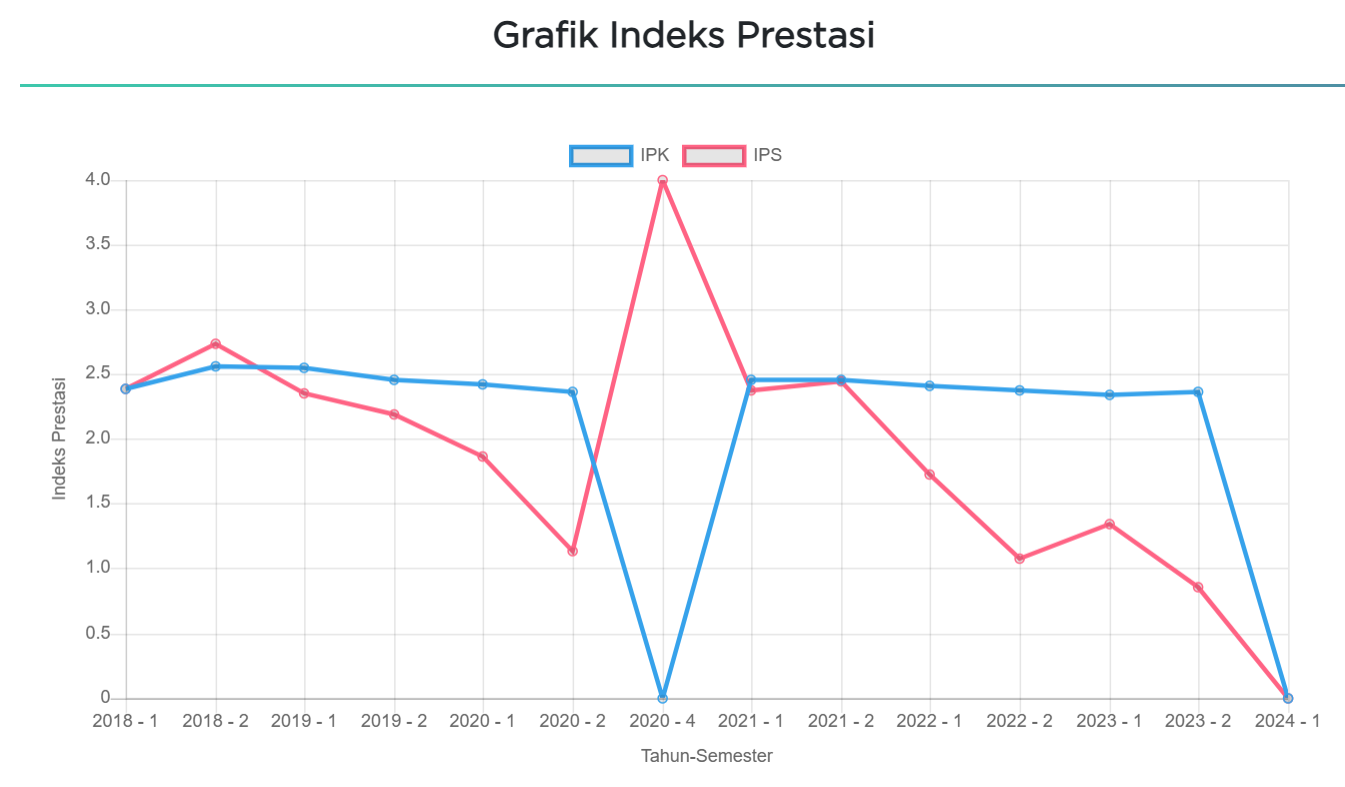
\includegraphics[width=0.5\linewidth]{Gambar/ContohLineChart.png}
    \caption{Contoh visualisasi dari perkembangan IPK dan IPS dengan menggunakan \textit{line plot}}
    \label{fig:contoh lineplot}
\end{figure}

\section{\textit{Tk Interface}}
\label{sec:tkinter}
\textit{Tk Interface} adalah sebuah antarmukan \textit{pyhton} standar untuk membuat aplikasi antarmuka grafis.~\cite{tkinter}
